\documentclass[review]{elsarticle}

\usepackage{hyperref}
\usepackage[table,xcdraw]{xcolor}
\usepackage{amsfonts}
\usepackage{amsmath}
\usepackage{amssymb}
\usepackage{amsthm}
\usepackage{graphicx}
\DeclareGraphicsExtensions{.pdf,.png,.jpg,.jpeg}
\graphicspath{{figures/}{./}}
\usepackage{multirow}
\usepackage{booktabs}
\usepackage{algorithm}
\usepackage{algorithmic}
\usepackage{natbib}
\usepackage{numcompress}
\bibliographystyle{model4-names}
\biboptions{authoryear}

\newtheorem{proposition}{Proposition}
\newtheorem{remark}{Remark}
\newtheorem{definition}{Definition}

\journal{Computer Methods and Programs in Biomedicine}

\begin{document}

\begin{frontmatter}

\title{Physics-Audited Soft-Tissue Digital Twins from Endoscopic Video:
Canonical Gaussian Fields, Simulation-in-the-Loop Elasticity Inversion,
and Parameter Provenance}

\author[1]{Ranyang~Li\corref{cor1}}
\author[2]{Nan~Wei}
\author[3]{Zhipeng~Lin}
\author[1]{Wufeng~Liu}
\author[1]{Chao~Fan}
\author[3]{Junjun~Pan\corref{cor1}}

\affiliation[1]{organization={Henan University of Technology},
                city={Zhengzhou},
                country={China}}
\affiliation[2]{organization={Henan Provincial People's Hospital},
                city={Zhengzhou},
                country={China}}
\affiliation[3]{organization={Beihang University},
                city={Beijing},
                country={China}}

\cortext[cor1]{Corresponding authors:
  \texttt{lry@haut.edu.cn} (R.~Li),
  \texttt{pan\_junjun@buaa.edu.cn} (J.~Pan)}

\begin{abstract}
\textbf{Objective.} Endoscopic scene reconstruction produces \emph{visual}
models of soft tissue, but surgical data science and patient-specific
planning need a \emph{physically simulable} twin --- and one that is honest
about what it knows. The mechanical parameters that make a twin simulable
(Young's modulus, Poisson ratio) are not directly observable from images,
yet existing methods either assign them silently or report them as if
measured. We present a pipeline that converts a monocular endoscopic video
into a simulable soft-tissue digital twin in which every physical parameter
carries an explicit, auditable provenance --- a capability that, to our
knowledge, no prior endoscopic-reconstruction method provides.
\textbf{Methods.} The twin is built in three stages on a single canonical
world-space Gaussian field: an optical-geometric stage reconstructs a
Gaussian BRDF field with tool-aware masking; a kinematic stage tracks
deformation with a constant-velocity model and divergence rollback; and a
mechanical-inversion stage recovers elastic properties by differentiable
simulation-in-the-loop inversion. Two ideas are central and new. A
force-scale propagation theorem proves that systematic force bias
propagates one-to-one into modulus bias while stiffness contrast is
force-scale-invariant, establishing what is knowable from video alone; and
a Bayesian provenance audit with a Laplace-posterior uncertainty study tags
every parameter as measured, estimated, or assumed, with calibrated
confidence.
\textbf{Results.} The reconstruction stage reaches 36.8\,dB and 34.1\,dB tissue-masked PSNR
on two EndoNeRF scenes and 26.6\,dB on real SCARED stereo data. The
mechanical-inversion stage is validated on four stages: a synthetic closed loop
(uniform modulus recovered to 0.01\% error; a $4\times$ stiff inclusion at
$3.19\times$ contrast); an independent FEM-generated benchmark (background
modulus recovered to a median error of 4.3\% across six scenarios, with
regime-dependent accuracy, and the recovered material predicts held-out
load cases within 4.1\% of oracle); a force-provenance study (background
error 4.1\,$\pm$\,4.0\%, contrast force-scale-immune); and a real
ultrasound phantom with compression-test ground truth (modulus contrast
$3.80\times$ vs.\ $3.56\times$, 6.9\% error, intervals containing both
ground-truth moduli).
\textbf{Conclusion.} The pipeline produces a validated, provenance-audited
soft-tissue digital twin from endoscopic video. Its distinguishing feature
is not only that the twin can be driven forward in a simulator, but that it
exposes, for every physical parameter, whether that parameter was measured,
estimated, or assumed --- turning an opaque reconstruction into a
trustworthy planning asset.
\end{abstract}

\begin{keyword}
digital twin \sep soft tissue \sep endoscopic video \sep 3D Gaussian
splatting \sep elasticity inversion \sep differentiable simulation \sep
parameter provenance \sep uncertainty quantification
\end{keyword}

\end{frontmatter}

%% ===================================================================
\section{Introduction}
\label{sec:intro}
%% ===================================================================

\begin{figure*}[htbp]
\centering
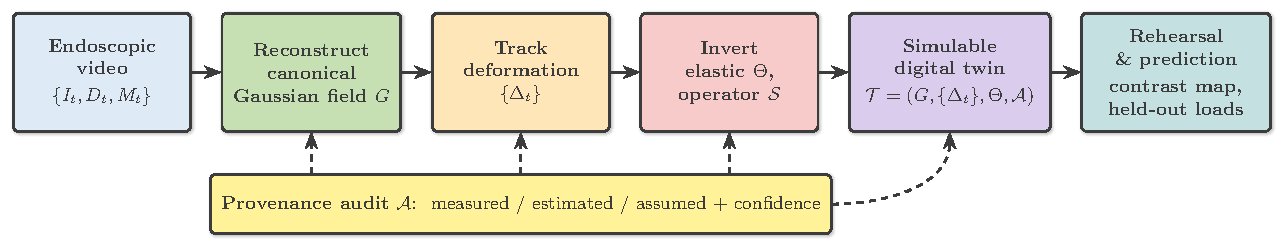
\includegraphics[width=\textwidth]{fig_pipeline.pdf}
\caption{Overall pipeline. The goal is to turn a monocular endoscopic
video into a soft-tissue digital twin that can be driven forward in a
physics simulator. The pipeline builds the twin in three stages on a
single canonical Gaussian field: the reconstruction stage fits the
optical-geometric field $G$ from the reference frame; the tracking stage
estimates the deformation sequence $\{\Delta_t\}$ on the fixed topology;
and the mechanical-inversion stage recovers the elastic parameters
$\Theta$ and the forward operator $\mathcal{S}$ by differentiable
simulation. The provenance audit $\mathcal{A}$ wraps the result, tagging
every physical parameter as measured, estimated, or assumed so a
downstream planner knows how much to trust it.}
\label{fig:pipeline}
\end{figure*}

Surgical data science, robot-assisted autonomy, and patient-specific
pre-operative planning all require a \emph{simulable} model of soft tissue:
a scene that can be loaded into a physics simulator and driven forward in
time to predict how the tissue will deform, contact, and respond to
instrument interaction. Such a model is fundamentally different from a
visual reconstruction. A reconstruction answers ``what does the tissue look
like''; a digital twin must also answer ``what will the tissue do''
\citep{landig2025,laubenbacher2024}. This paper presents a pipeline that
builds exactly such a twin: it takes a monocular endoscopic video sequence
as input and produces a physically simulable soft-tissue digital twin as
output (Fig.~\ref{fig:pipeline}).

The clinical motivation is concrete. In robot-assisted surgery, a
patient-specific twin would allow a surgeon or an autonomous controller to
rehearse a retraction, dissection, or suturing plan in simulation before
touching tissue. In surgical training, a library of twins with known
mechanical properties would enable realistic haptic rehearsal. In
image-guided therapy, a twin synchronized with the live endoscopic feed
could predict out-of-view deformation. All of these depend not on
photorealism but on the twin's \emph{physical parameters} being correct ---
and, just as importantly, on the user knowing how much to trust them.

The core difficulty is that geometry and appearance are observable from
images, while mechanical parameters --- Young's modulus $E$, Poisson ratio
$\nu$, viscosity --- are not. A pixel records radiance, not stress. A
mechanical parameter can only be obtained in two ways: (a) it is looked up
from a tissue-class prior (an assumption), or (b) it is inferred by
observing deformation under known loading (a measurement, subject to the
identifiability limits of the loading). Prior reconstruction work either
ignores this distinction by assigning constants silently, or over-claims by
reporting $E$ as if it were measured. Neither is acceptable for a twin that
will drive clinical decisions, because a simulator fed with unfounded
constants produces plausible-looking but physically wrong predictions ---
which is worse than no twin at all.

Our answer has two linked parts (Fig.~\ref{fig:pipeline} and
Fig.~\ref{fig:architecture}). First, we build the twin in three stages that
share a single canonical world-space 3D Gaussian field, so that appearance,
motion, and mechanics live on the same primitives: an optical-geometric
stage reconstructs the field $G$, a tracking stage tracks the deformation
sequence $\{\Delta_t\}$, and a mechanical stage recovers the elastic
parameters $\Theta$ and the forward operator $\mathcal{S}$. Second, and
central to the paper, we attach a \emph{provenance audit} to the twin:
every physical parameter is tagged as \emph{measured} (recovered from
observed deformation under known loading), \emph{estimated} (inferred from
weaker evidence), or \emph{assumed} (taken from a tissue-class table), with
a confidence. A downstream planner can then weight the twin's predictions
by how much each parameter can be trusted, which aligns with the broader
trustworthy-health-AI agenda that clinical models must expose what is
measured versus assumed \citep{topol2019,landig2025}.

The significance of building the twin this way is twofold. Practically, it
turns the endoscopic video that every procedure already produces into a
rehearsal asset: the surgeon can simulate the next interaction and inspect
a stiffness-contrast map that may localize a stiff tumor margin.
Theoretically, it clarifies what can and cannot be known from video alone:
a force-scale propagation theorem (Proposition~\ref{prop:forcescale})
proves that absolute modulus is bounded by force-sensing accuracy while
stiffness contrast is force-scale-invariant, so the twin reports contrast
as the robust measured quantity and absolute modulus with honest intervals.
The paper advances this goal in four ways. We introduce a three-stage
architecture that reuses a single canonical Gaussian field as the shared
substrate for optical reconstruction, deformation tracking, and mechanical
inversion, supported by tool-aware tissue supervision and a
divergence-robust tracker (Sec.~\ref{sec:method}). We prove a force-scale
propagation theorem (Proposition~\ref{prop:forcescale}) that formalizes
what is knowable from video alone. We attach a parameter-provenance audit
that tags every physical parameter as measured, estimated, or assumed with
a calibrated confidence (Sec.~\ref{sec:uq}). And we validate the pipeline
on a four-stage protocol that runs from a synthetic closed loop to a real
phantom with independent compression-test ground truth
(Sec.~\ref{sec:experiments}).

Across two EndoNeRF scenes and the SCARED stereo dataset, the
optical-geometric stage reconstructs tissue at 26.6--36.8\,dB tissue-masked
PSNR. The kinematic stage tracks deformation robustly where a naive tracker
diverges. The mechanical stage recovers uniform modulus to 0.01\% error in a
synthetic closed loop, background modulus to a median of 4.3\% error on an
independent FEM benchmark, and modulus contrast to 6.9\% error on a real
ultrasound phantom with independent compression-test ground truth. We claim
a working three-stage pipeline, a formal account of parameter provenance, a
force-scale propagation theorem with empirical confirmation, and a
staged validation reaching a real phantom; we do \emph{not} claim
absolute-modulus recovery on real tissue without force sensing (we show
contrast instead), state-of-the-art reconstruction, or clinical readiness.

The rest of the paper is organized as follows. Section~\ref{sec:related}
reviews related work. Section~\ref{sec:method} presents the twin and its
three stages, the force-scale theorem, and the audit.
Section~\ref{sec:experiments} reports the staged validation and ablations.
Section~\ref{sec:discussion} discusses measured versus assumed parameters,
limits, and clinical translation. Section~\ref{sec:conclusion} concludes.

%% ===================================================================
\section{Related work}
\label{sec:related}
%% ===================================================================

We position this work along five directions and summarize the comparison in
Table~\ref{tab:position}.

\begin{table*}[htbp]
\centering
\caption{Positioning against representative related work.}
\label{tab:position}
\small
\begin{tabular}{@{}p{0.16\linewidth}p{0.20\linewidth}p{0.16\linewidth}p{0.16\linewidth}p{0.16\linewidth}@{}}
\toprule
Method & Output & Mechanics & Provenance & Validated on \\
\midrule
EndoNeRF \citep{endonerf} & appearance + geometry & none & none & EndoNeRF \\
EndoSurf \citep{endosurf} & surface + appearance & none & none & stereo endoscopy \\
EndoGaussian \citep{endogaussian} & appearance + geometry & none & none & EndoNeRF \\
PAC-NeRF \citep{pacnerf} & geometry + system ID & $E$, known force & implicit & synthetic + objects \\
PhysDreamer \citep{physdreamer} & relative stiffness & relative $E$ & implicit & static objects \\
PhysGaussian \citep{physgaussian} & dynamics & MPM, manual $E$ & none & synthetic \\
\textbf{Ours} & \textbf{simulable twin} & $E$, $\nu$, viscosity & \textbf{explicit audit} & \textbf{EndoNeRF + SCARED + FEM + phantom} \\
\bottomrule
\end{tabular}
\end{table*}

\subsection{Medical digital twins}
Digital twins originated in industry, where a constantly updating virtual
copy enables analysis, simulation, and prediction of a real-world asset
\citep{tao2019,fuller2020}, and are increasingly studied as a route to
precision medicine. Recent frameworks decompose a medical twin into the
patient, the data connection, the patient-in-silico model, the interface,
and twin synchronisation \citep{landig2025,laubenbacher2024}. The
cardiology community has produced the most mature examples, with
electrophysiology heart twins used to plan ablation and resynchronization
therapy; oncology has produced tumor-growth twins coupling imaging with
reaction--diffusion models; and epidemiology has produced population-level
twins for policy testing. These share a common structure --- a mechanistic
or learned patient-in-silico model synchronized with patient data --- but
their state variables are compartmental, hemodynamic, or cellular rather
than mechanical. Intra-operative soft-tissue twins built from endoscopic
video remain largely unexplored, and none of the existing frameworks
addresses the provenance of the twin's physical parameters. Our work brings
an explicit measured/estimated/assumed audit into a soft-tissue twin from
endoscopic video, and our synchronization loop (Sec.~\ref{sec:sync})
follows the twin-synchronisation component of the framework of
\citet{landig2025}.

\subsection{Endoscopic scene reconstruction}
EndoNeRF \citep{endonerf} introduced neural radiance fields \citep{nerf}
for deformable endoscopic scenes, demonstrating novel-view synthesis of
tissue deformation by conditioning a radiance field on a learned
deformation code per frame. EndoSurf \citep{endosurf} improved surface
fidelity by combining a neural signed-distance field with a surface-aware
rendering loss, yielding cleaner tissue boundaries. A line of
Gaussian-splatting methods \citep{gaussiansplatting} --- EndoGaussian
\citep{endogaussian}, LGS, and deformable-Gaussian variants --- replaced
the implicit field with anisotropic 3D Gaussians, gaining an order of
magnitude in rendering speed and enabling per-primitive appearance. These
methods reconstruct appearance and geometry but do not recover physical
parameters, and their output cannot be loaded into a physics simulator.
Complementary lines address camera tracking and mapping in endoscopy, from
stereo correspondence \citep{allan2021} and robust pose estimation
\citep{hayoz2023} to deformable SLAM \citep{defslam}, and inverse-rendering
methods recover relightable appearance with BRDF decomposition
\citep{gsir2024,relightable3dgs}, but none of these recover mechanical
parameters either. Our reconstruction stage shares the Gaussian representation but adds a
physically constrained BRDF (Sec.~\ref{sec:tier1}) and, more importantly,
uses the field as the substrate for the kinematic and mechanical stages
rather than as an end in itself. The tool-aware masking of
Sec.~\ref{sec:tier1} is also a reconstruction-side contribution: these
methods typically reconstruct the whole frame including tools, whereas we
show that correct tissue-only supervision is worth ${\sim}25$\,dB.

\subsection{Physics-aware reconstruction}
A growing line of work couples neural reconstruction with physics.
PAC-NeRF \citep{pacnerf} performs system identification from multi-view
video with known forces, recovering material parameters of household
objects by matching a differentiable continuum simulator to observed
motion; its key requirement is a measured force, which is rarely available
in endoscopy. PhysDreamer \citep{physdreamer} uses a video diffusion prior
to estimate the relative stiffness of static objects, trading absolute
accuracy for the ability to work from a single video. PhysGaussian
\citep{physgaussian} embeds the Material Point Method into Gaussians for
generative dynamics but requires manually supplied material parameters, so
the physics is imposed rather than recovered. Spring-Gaus and similar
variants attach spring models to Gaussians for elastic dynamics
\citep{springgaus,physicallyembodied}, and graph-network simulators learn
complex physics from data \citep{sanchezgonzalez2020}. These works
demonstrate that physics can be coupled with learned reconstruction, but
they either assume known forces, recover only relative stiffness, or
require manual parameters --- and none audits the provenance of the
resulting values. We target endoscopic soft tissue, recover absolute
modulus where identifiable, and audit every parameter; our
Proposition~\ref{prop:forcescale} additionally clarifies, at the level of
theory, why the known-force requirement of PAC-NeRF is the binding
constraint on absolute modulus.

\subsection{Elastography}
Quasi-static elastography recovers modulus contrast from deformation under
a shared-stress approximation \citep{ophir1991,wells2011,sigrist2017}, and
is clinically established for liver fibrosis staging and tumor detection.
The method tracks the axial strain induced by a small compression; under
the assumption that the stress is approximately uniform across a region,
the ratio of strains in two regions approximates the inverse ratio of their
moduli, so a stiff inclusion stands out as a low-strain region. Its central
limitation --- that without force measurement only contrast, not absolute
modulus, is identifiable --- is one we adopt explicitly rather than
circumvent. Our force-scale propagation theorem
(Proposition~\ref{prop:forcescale}) formalizes exactly this point, and our
audit reports contrast as the robust measured quantity. The \'ETS phantom
experiment of Sec.~\ref{sec:experiments} places our video-derived contrast
within the accuracy range expected of clinical elastography.

\subsection{Differentiable simulation and uncertainty}
Differentiable physics --- differentiable FEM, MPM, and mass--spring
solvers --- enables gradient-based parameter inversion through a simulator
\citep{pacnerf,physgaussian,hu2020difftaichi,sanchezgonzalez2020}. We use a
differentiable Neo-Hookean FEM for the main inversion and a fast
mass--spring surrogate for synthetic closed-loop studies, and we quantify
the surrogate's inadequacy (82\% forward error) to justify the FEM choice.
On the uncertainty side, Laplace approximations and Monte-Carlo propagation
are standard \citep{kendall2017,gal2016,lakshminarayanan2017}; our
contribution is to use them to \emph{flag} unidentifiable parameters rather
than to decorate point estimates.

\subsection{Gaps and our response}
\label{sec:gaps}
Synthesizing the five directions, four gaps define where this work sits.
(G1) \emph{From reconstruction to simulation}: endoscopic reconstruction
produces appearance and geometry but no forward operator; we add kinematic
and mechanical stages so the same Gaussian field becomes simulable.
(G2) \emph{From assigned to recovered mechanics}: existing physics-aware
methods assign parameters manually or recover only relative stiffness; we
recover absolute modulus where identifiable and say so when it is not.
(G3) \emph{From silent to audited parameters}: no prior method exposes
whether a parameter is measured, estimated, or assumed; our audit makes
this explicit. (G4) \emph{From single-setting to ladder validation}:
mechanics papers typically validate in one setting; we validate on a ladder
from synthetic to a real phantom with independent ground truth. Each
contribution in Sec.~\ref{sec:intro} maps to one of these gaps.

%% ===================================================================
\section{Method}
\label{sec:method}
%% ===================================================================

\begin{figure*}[htbp]
\centering
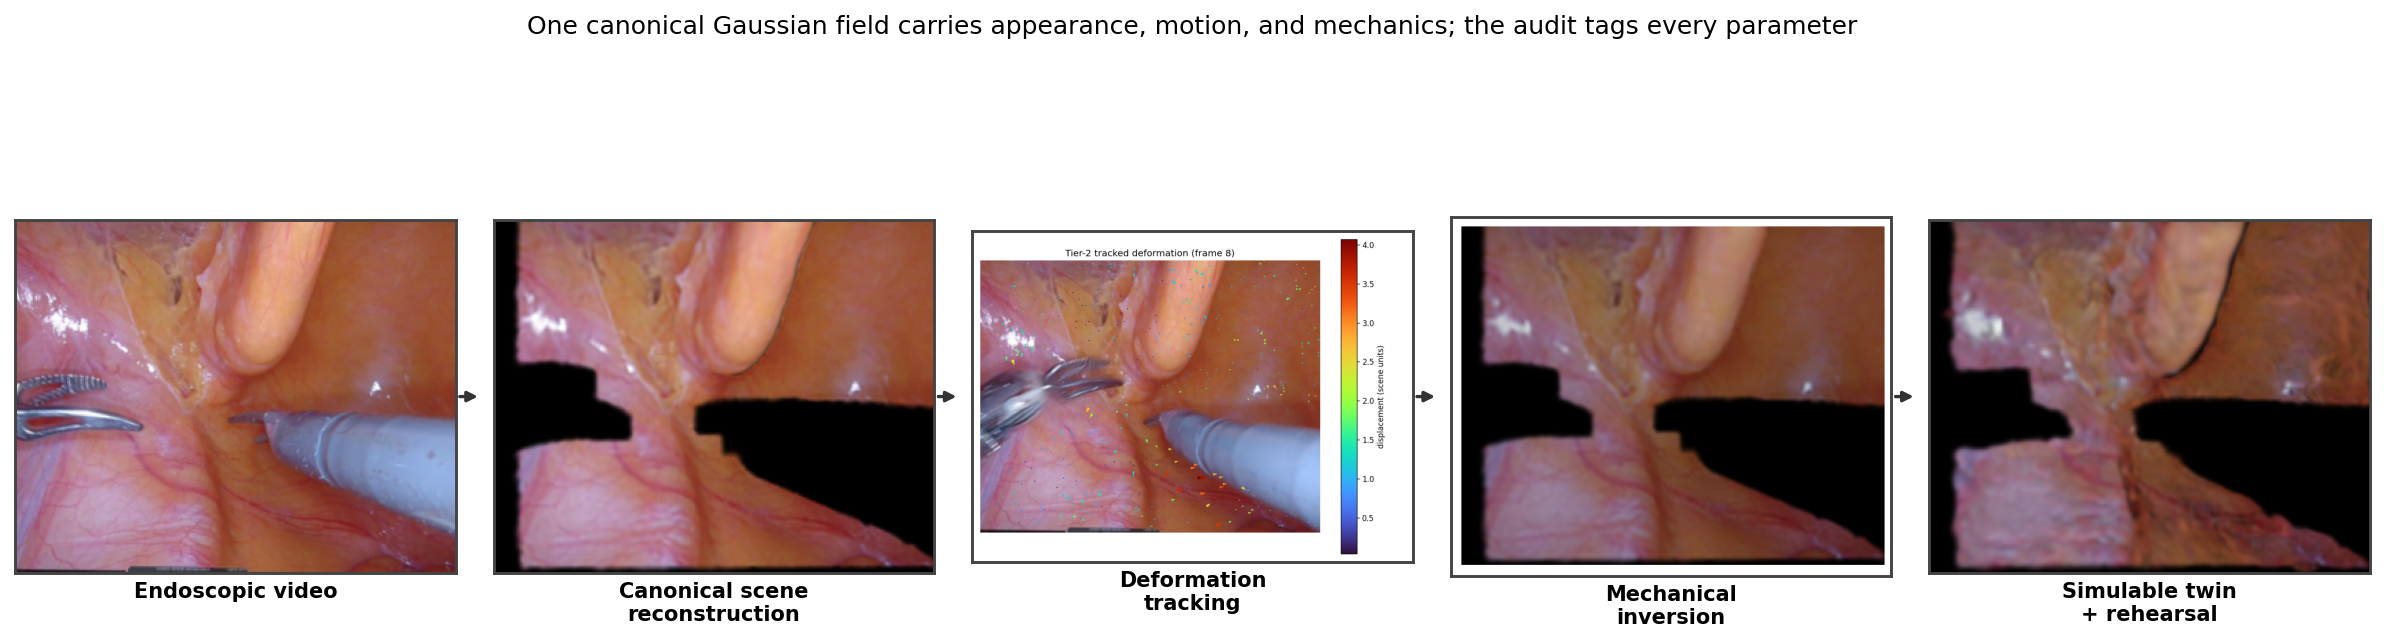
\includegraphics[width=\textwidth]{fig_architecture_results.png}
\caption{Model architecture, shown through the actual outputs of each
stage. Reading left to right: the endoscopic video is reconstructed into
a canonical Gaussian field (optical output), tracked through deformation
(kinematic output), and inverted for its mechanical parameters
(mechanical output), yielding a simulable twin that can be driven forward
for rehearsal. The provenance audit tags every parameter.}
\label{fig:architecture}
\end{figure*}

\subsection{The soft-tissue digital twin}
\label{sec:twin}
\begin{definition}[Soft-tissue digital twin]
\label{def:twin}
A soft-tissue digital twin is a tuple
$\mathcal{T} = (G, \{\Delta_t\}, \Theta, \mathcal{A})$, where $G$ is a
canonical geometric and optical scene representation, $\{\Delta_t\}$ is a
deformation sequence on $G$, $\Theta$ is a set of physical parameters
(elastic, viscous, inertial, optical), and $\mathcal{A}$ is an audit map
assigning to each $\theta \in \Theta$ a provenance tag and confidence. The
twin is \emph{simulable} if there exists a forward operator
$\mathcal{S} : (G, \Theta, f) \mapsto u$ mapping a load $f$ to a
deformation $u$, and it is \emph{audited} if $\mathcal{A}$ is complete
(every $\theta$ is tagged).
\end{definition}

The goal is to construct an audited, simulable $\mathcal{T}$ from
endoscopic video alone. Fig.~\ref{fig:architecture} shows the architecture:
one canonical Gaussian field $G$ is the shared substrate, built by the reconstruction stage,
deformed by the tracking stage, and given mechanics by the mechanical-inversion stage, and the audit wraps the
resulting parameters. The input is a sequence of endoscopic frames
$\{I_t\}_{t=1}^{T}$ with per-frame depth maps $D_t$ and tool masks $M_t$;
the output is the twin $\mathcal{T}$.
Fig.~\ref{fig:twin_complete} shows a complete input$\to$twin$\to$output
result on a real endoscopic sequence, which the method subsections below
construct stage by stage. Table~\ref{tab:notation} lists the
main symbols.

\begin{table}[htbp]
\centering
\caption{Main symbols.}
\label{tab:notation}
\small
\begin{tabular}{@{}p{0.28\linewidth}p{0.64\linewidth}@{}}
\toprule
Symbol & Meaning \\
\midrule
$I_t, D_t, M_t$ & frame image, depth map, tool mask \\
$G=\{g_i\}_{i=1}^{N}$ & canonical Gaussian field, $N$ primitives \\
$\mathbf{x}_i, \Sigma_i, o_i, \mathbf{n}_i$ & position, covariance, opacity, normal of $g_i$ \\
$\rho_d,\rho_s,\alpha,m,a$ & diffuse, specular, roughness, metalness, absorption \\
$\Delta_t$ & per-Gaussian displacement at frame $t$ \\
$E, \nu$ & Young's modulus (Pa), Poisson ratio \\
$u, f$ & nodal displacement, external force \\
$\Omega$ & tissue pixel set \\
$E_{bg}, E_{incl}$ & background / inclusion modulus \\
\bottomrule
\end{tabular}
\end{table}

\subsection{Canonical scene reconstruction}
\label{sec:tier1}
The reconstruction stage builds $G$. Each Gaussian $g_i$ stores a position
$\mathbf{x}_i \in \mathbb{R}^3$, an anisotropic covariance
$\Sigma_i = R(q_i)\,\mathrm{diag}(s_i^2)\,R(q_i)^{\top}$ with rotation
quaternion $q_i$ and scale $s_i$, an opacity $o_i \in [0,1]$, a unit normal
$\mathbf{n}_i$, and BRDF parameters $(\rho_d, \rho_s, \alpha, m, a)$. A
softmax energy budget enforces a partition of unity,
\begin{equation}
\rho_d + \rho_s + a = 1, \qquad \rho_d,\rho_s,a \ge 0,
\label{eq:budget}
\end{equation}
so that no primitive reflects more energy than it receives. Images are
formed by front-to-back alpha compositing,
\begin{equation}
\hat{I} = \sum_{i=1}^{N} c_i\,\alpha_i \prod_{j<i}(1-\alpha_j),
\label{eq:render}
\end{equation}
where $c_i$ is the shaded color of $g_i$ and $\alpha_i$ its projected
opacity. The shaded color follows a Cook--Torrance microfacet BRDF
\citep{cooktorrance} split into a diffuse and a specular lobe,
\begin{equation}
c_i = \underbrace{\frac{\rho_d}{\pi}\,E_d}_{\text{diffuse}}
+ \underbrace{\rho_s\,\frac{D(\alpha)\,G\,F}{4\,(\mathbf{n}\cdot\mathbf{l})(\mathbf{n}\cdot\mathbf{v})}}_{\text{specular}},
\label{eq:cooktorrance}
\end{equation}
where $E_d$ is the diffuse irradiance, $D(\alpha)$ the GGX normal
distribution, $G$ the Smith geometry term, $F$ the Schlick Fresnel term,
$\mathbf{l}$ the light direction, and $\mathbf{v}$ the view direction. The
highlight-free diffuse image is obtained by setting the specular lobe to
zero.

A key endoscopic adaptation concerns the supervision mask. The EndoNeRF
\texttt{masks/} channel marks \emph{tools}, not tissue, and tools have no
valid depth. We therefore define the tissue pixel set as
\begin{equation}
\Omega = \{(u,v) : D(u,v) > \epsilon \} \setminus M,
\label{eq:mask}
\end{equation}
with $\epsilon$ a small depth-validity threshold, and supervise only on
$\Omega$. Supervising on the tool mask instead of $\Omega$ degrades
reconstruction by ${\sim}25$\,dB (Table~\ref{tab:ablation}). The reconstruction-stage
objective is
\begin{equation}
\mathcal{L}_1 = \lambda_{ph}\,\mathcal{L}_{photo} + \lambda_d\,\mathcal{L}_{depth} + \lambda_\alpha\,\mathcal{L}_{\alpha},
\label{eq:tier1loss}
\end{equation}
with non-negative weights $\lambda_{ph},\lambda_d,\lambda_\alpha$, a masked
$L_1 + 0.5\,L_2$ photometric term $\mathcal{L}_{photo}$ on $\Omega$, a
depth $L_1$ term $\mathcal{L}_{depth}$ on $\Omega$, and an alpha BCE term
$\mathcal{L}_{\alpha}$ toward the tissue mask. Lighting is an
endoscope-co-located directional light plus a strong ambient
spherical-harmonic lobe, so appearance approximates albedo; a learnable
exposure closes the residual gap.

\subsection{Deformation tracking}
\label{sec:tier2}
The tracking stage builds $\{\Delta_t\}$ by tracking a per-Gaussian displacement
$\Delta_t \in \mathbb{R}^{N \times 3}$ on the canonical topology, keeping
correspondences fixed across time. Fixed correspondence is what
distinguishes a twin from a per-frame rebuild: the same primitive is
followed through time, so its trajectory is a boundary condition. Naive
inertia-only tracking (penalizing $\|\Delta_t - \Delta_{t-1}\|^2$)
occasionally diverges on ambiguous frames. We therefore optimize
\begin{align}
\Delta_t^* = \arg\min_{\Delta}\ \ & \mathcal{L}_{photo}(\Delta)
+ \lambda_s \sum_{i=1}^{N} \big\| \Delta_i - \bar{\Delta}_{\mathcal{N}(i)} \big\|^2 \nonumber\\
& + \lambda_a \big\| \Delta - 2\Delta_{t-1} + \Delta_{t-2} \big\|^2,
\label{eq:track}
\end{align}
initialized from the constant-velocity extrapolation
$\Delta_t^{(0)} = 2\Delta_{t-1} - \Delta_{t-2}$. The second term is a
$k$-nearest-neighbor Laplacian smoothness over the Gaussian graph; the
third is an acceleration prior that penalizes changes in velocity rather
than velocity itself. A per-frame step cap constrains
$\mathrm{mean}|\Delta_t| \le 3\times$ the running median of past steps, and
a divergence rollback re-optimizes at half learning rate if the final loss
exceeds $3\times$ the previous frame's, else keeps $\Delta_{t-1}$ and flags
the frame. The output is a sequence of replayable boundary conditions.

\subsection{Mechanical parameter inversion}
\label{sec:tier3}
The mechanical-inversion stage builds $\Theta$ and the forward operator $\mathcal{S}$. Soft tissue
is modeled as a quasi-static continuum in equilibrium,
\begin{equation}
R(u; E, \nu, f) = f_{int}(u; E, \nu) - f_{ext} = 0,
\label{eq:equilibrium}
\end{equation}
where $f_{int}$ is the internal elastic force and $f_{ext}$ the applied
load. We invert $E$ by gradient descent through a differentiable forward
solver,
\begin{equation}
E^* = \arg\min_{E} \sum_{t} \big\| u(E, \nu, f_t) - u_t^{obs} \big\|_{\Omega}^{2} + \lambda\,\mathcal{R}(E),
\label{eq:inversion}
\end{equation}
where $u(E,\nu,f_t)$ is the simulated displacement under load $f_t$,
$u_t^{obs}$ the observed deformation, and $\mathcal{R}(E)$ a regularizer
(log-normal prior plus spatial smoothness). Two forward models are used: a
mass--spring lattice (structural and shear springs with stiffness
$k = E\,h$, $h$ the lattice spacing) for synthetic closed-loop studies, and
a differentiable Neo-Hookean FEM \citep{holzapfel2000,ogden1997,fung1993}
with strain-energy density
\begin{equation}
\Psi(F) = \frac{\mu}{2}\big(\mathrm{tr}(F^{\top}F) - 3\big) - \mu\,\log J + \frac{\lambda}{2}(\log J)^2,
\label{eq:neohookean}
\end{equation}
where $F$ is the deformation gradient, $J = \det F$, and
$\mu = E/(2(1+\nu))$, $\lambda = E\nu/((1+\nu)(1-2\nu))$ are the Lam\'e
parameters. The FEM solve uses Newton iteration with load stepping and warm
starts, and gradients are obtained by the implicit-function theorem through
the equilibrium. A kPa-scale log-normal tissue database (liver, fat,
muscle, skin, tumor; Table~\ref{tab:tissue}) with near-incompressible $\nu$
and constitutive-model tags (Neo-Hookean / Mooney--Rivlin
\citep{rivlin1948} / Ogden \citep{ogden1997}) provides priors; the tissue
class is selected by a heuristic classifier on the optical signature
(perfusion hue and specular wetness), which selects the prior class only,
never the mechanical values.

\begin{table}[htbp]
\centering
\caption{Soft-tissue priors (kPa-scale, log-normal $E$).}
\label{tab:tissue}
\footnotesize
\begin{tabular}{@{}p{0.22\linewidth}cccc@{}}
\toprule
Tissue & median $E$ (kPa) & $\nu$ & density (kg/m$^3$) & model \\
\midrule
liver & 6 & 0.48 & 1060 & Neo-Hookean \\
fat & 2 & 0.45 & 950 & Neo-Hookean \\
muscle & 20 & 0.49 & 1060 & Mooney--Rivlin \\
skin & 80 & 0.48 & 1100 & Ogden \\
tumor & 30 & 0.48 & 1050 & Neo-Hookean \\
generic soft tissue & 10 & 0.47 & 1040 & Neo-Hookean \\
\bottomrule
\end{tabular}
\end{table}

\subsection{Force-scale propagation}
\label{sec:forcescale}
The following result is the theoretical basis for reporting stiffness
contrast as the robust measured quantity.

\begin{proposition}[Force-scale propagation]
\label{prop:forcescale}
Consider a linear-elastic body in equilibrium, $K(E)\,u = f$, with
stiffness matrix linear in $E$, $K(E) = E\,\tilde{K}$, where $\tilde{K}$ is
independent of $E$. Then (i) a global force scale error $f \to \beta f$ is
exactly compensated by $E \to \beta E$, i.e.\ the equilibrium displacement
is unchanged:
\begin{equation}
u(\beta E, \nu, \beta f) = u(E, \nu, f);
\label{eq:scale}
\end{equation}
and (ii) the stiffness contrast $E_{incl}/E_{bg}$ between any two regions
is invariant to any global force scale $\beta$.
\end{proposition}

\begin{proof}
For (i), substitute into the equilibrium:
\begin{equation*}
K(\beta E)\,u(\beta E, \nu, \beta f) = \beta E\,\tilde{K}\,u(\beta E, \nu, \beta f) = \beta f.
\end{equation*}
Dividing by $\beta$ gives $E\,\tilde{K}\,u(\beta E, \nu, \beta f) = f$,
whose solution is $u(E,\nu,f)$ by definition, so
$u(\beta E, \nu, \beta f) = u(E, \nu, f)$. For (ii), the contrast is
$(\beta E_{incl})/(\beta E_{bg}) = E_{incl}/E_{bg}$, and the factor $\beta$
cancels.
\end{proof}

\begin{remark}
\label{rem:nonlinear}
The argument is exact for linear elasticity and holds approximately for the
Neo-Hookean model at the moderate strains considered here; the systematic
sweep in Sec.~\ref{sec:force} confirms it empirically (force scale
0.80--1.20 $\to$ $E_{bg}$ ratio 0.846--1.110). Consequence (i) means
absolute $E$ is bounded by the force estimator's systematic accuracy;
consequence (ii) means contrast is robust to any global force scale.
\end{remark}

\paragraph{The force estimator}
\label{sec:forceest}
The force $f$ that drives the mechanical inversion is provided by a
video-based force estimator (prior work \citep{smallbowelforce}, not our
contribution), whose architecture is shown in
Fig.~\ref{fig:forcenet}. It maps a short endoscopic video window
$V \in \mathbb{R}^{3 \times T \times H \times W}$ ($T$ frames of
$H \times W$ RGB) to a scalar interaction force $\hat{f}$. A 3D-ResNet
(R3D-18 \citep{r3d}, pretrained on Kinetics-400) extracts a spatiotemporal
feature, and a two-layer perceptron head regresses the force:
\begin{equation}
\hat{f} = g_{\phi}(V) = w_{2}^{\top}\,\sigma\!\left(W_{1}\,\phi(V) + b_{1}\right) + b_{2},
\label{eq:forcenet}
\end{equation}
where $\phi(V) \in \mathbb{R}^{512}$ is the R3D-18 backbone feature (global
average-pooled), $\sigma$ is ReLU, $W_{1} \in \mathbb{R}^{512 \times 512}$,
and $w_{2} \in \mathbb{R}^{512}$. The backbone is frozen except for the last
two residual stages, which are fine-tuned. The estimator is trained with an
$\ell_{2}$ regression loss against instrumented force measurements
$f^{\star}$:
\begin{equation}
\mathcal{L}_{\text{force}} = \frac{1}{N}\sum_{i=1}^{N}\left\lVert g_{\phi}(V_{i}) - f^{\star}_{i}\right\rVert_{2}^{2}.
\label{eq:forceloss}
\end{equation}
We do not retrain this estimator; we use only its empirical error model ---
a systematic scale factor $0.949 \pm 0.140$ and MAE $0.295$\,N measured on
the small-bowel retraction benchmark --- which
Proposition~\ref{prop:forcescale} transports onto the modulus estimate.

\begin{figure}[htbp]
\centering
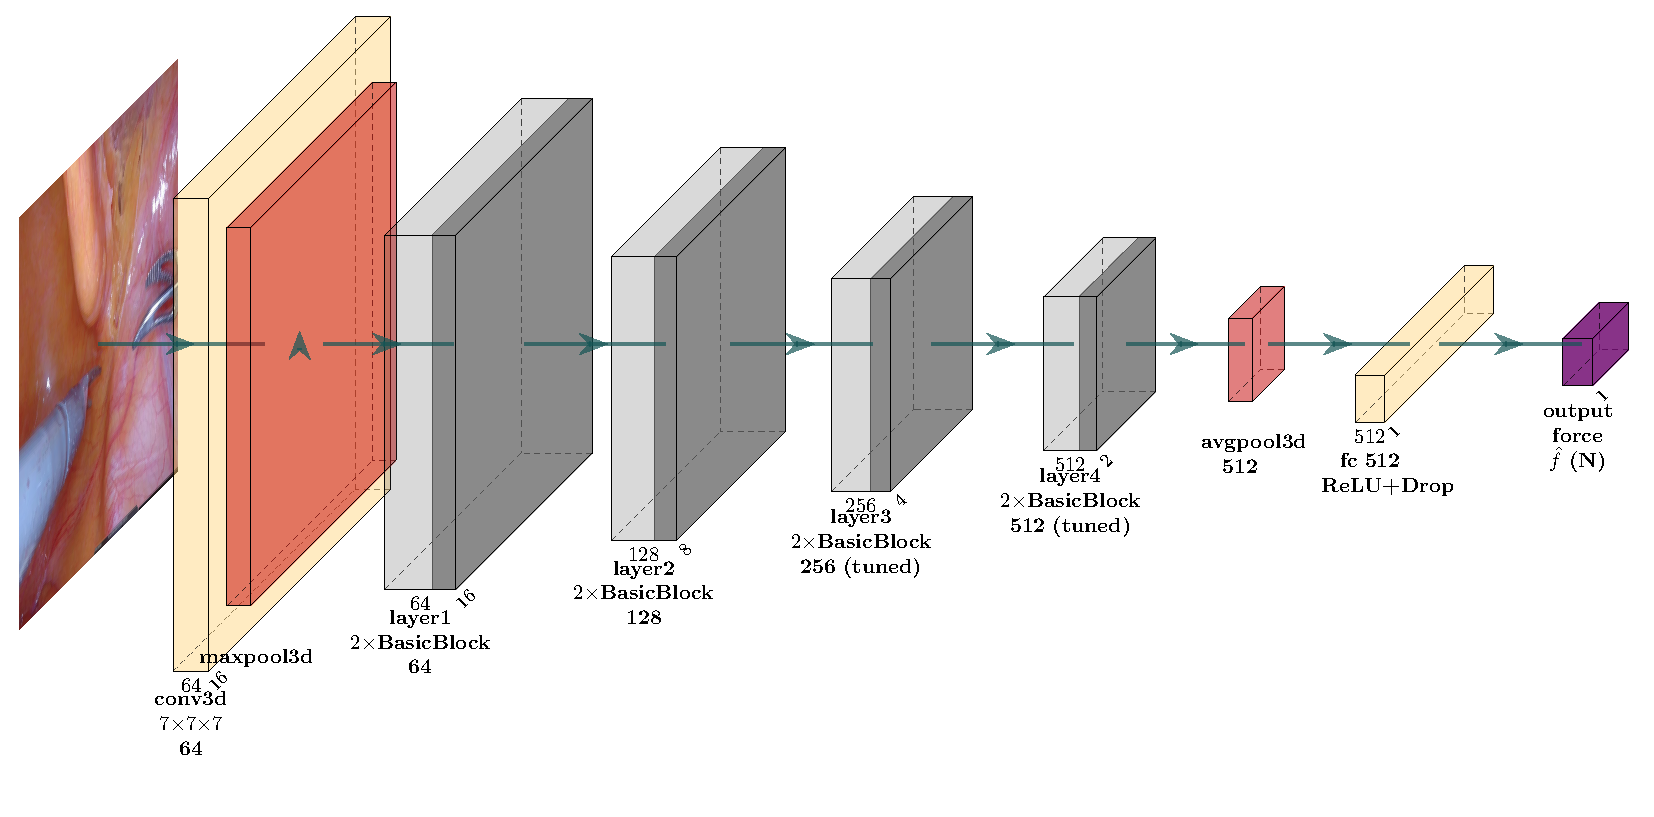
\includegraphics[width=\linewidth]{fig_forcenet.pdf}
\caption{Architecture of the video-based force estimator
(Eq.~\ref{eq:forcenet}, prior work \citep{smallbowelforce}). A 3D-ResNet
(R3D-18) backbone processes the video clip $3 \times T \times H \times W$
through a 3D-convolution stem and four residual stages (only the last two
are fine-tuned), followed by global average pooling and a two-layer
regressor head (Eq.~\ref{eq:forceloss}) that outputs the scalar force
$\hat{f}$.}
\label{fig:forcenet}
\end{figure}

\subsection{The provenance audit}
\label{sec:uq}
\begin{definition}[Parameter provenance]
\label{def:provenance}
A physical parameter $\theta$ carries a provenance tag
$\tau(\theta) \in \{\text{measured}, \text{estimated}, \text{assumed}\}$ and
a confidence $c(\theta) \in [0,1]$. $\theta$ is \emph{measured} if it was
recovered from observed deformation under known loading; \emph{estimated}
if it was inferred from weaker evidence (optical signature or deformation
without force) via Bayesian update; and \emph{assumed} if it was taken from
a tissue-class table.
\end{definition}

Young's modulus uses a log-normal prior
$\log E \sim \mathcal{N}(\mu_0, \sigma_0^2)$, appropriate because tissue
stiffness spans orders of magnitude and must stay positive. A
Gaussian--Gaussian update combines the prior with deformation evidence in
closed form,
\begin{equation}
\sigma_{post}^{-2} = \sigma_0^{-2} + \sigma_{obs}^{-2}, \qquad
\mu_{post} = \sigma_{post}^{2}\left(\frac{\mu_0}{\sigma_0^{2}} + \frac{\mu_{obs}}{\sigma_{obs}^{2}}\right),
\label{eq:bayes}
\end{equation}
where $(\mu_{obs}, \sigma_{obs})$ summarize the deformation evidence. The
confidence is the fractional posterior narrowing,
$c = 1 - \sigma_{post}/\sigma_0$. For uncertainty propagation, a Laplace
approximation $p(\log E \mid \text{data}) \approx \mathcal{N}(\log E^*, H^{-1})$
with $H$ the Hessian of the negative log-likelihood at the optimum is
sampled by Monte Carlo through the simulator to a 95\% prediction interval.

\subsection{Using the twin}
\label{sec:sync}
A digital twin is not a one-shot reconstruction but a continuously updated
copy \citep{landig2025}. Synchronization is the tracking loop: as each new
frame arrives, the tracker updates $\{\Delta_t\}$ on the fixed canonical
topology, and the mechanical stage reuses the accumulated deformation as
additional inversion evidence, so the twin stays current at interactive
rates and its confidence improves as more of the procedure is observed.
Once constructed, the twin is used by driving $\mathcal{S}$ with new loads:
given a planned instrument trajectory $\{f_t^{plan}\}$, the simulator
produces the predicted deformation $\{u(E^*, \nu, f_t^{plan})\}$, which can
be rendered through the reconstruction-stage field for visual rehearsal or post-processed
for quantities of interest (contact force, strain energy density, margin
strain). The audit modulates how these predictions are presented:
predictions that depend on \emph{measured} parameters are shown with tight
intervals, those depending on \emph{assumed} parameters with wide ones.

\begin{remark}[No neural network in the core method]
\label{rem:networkfree}
The core of the method is physics-based optimization, not a learned neural
network: the Gaussian field is a set of per-primitive physical parameters
optimized in place, the renderer is a differentiable rasterizer, and the
mechanical inversion is gradient descent on physical parameters through a
differentiable simulator. The only learned component is the video-based
force estimator used as a prior in the force-provenance study
(Sec.~\ref{sec:force}), which is taken from prior work
\citep{smallbowelforce} and is not our contribution. This network-free
design is deliberate: it keeps the twin interpretable, requires no training
data, and makes every parameter physically meaningful --- which is what the
audit framework is built on.
\end{remark}

%% ===================================================================
\section{Experiments}
\label{sec:experiments}
%% ===================================================================

\subsection{Experimental setup}
\label{sec:setup}

\paragraph{Datasets.}
Table~\ref{tab:datasets} summarizes the four datasets, which span
increasingly realistic validation settings.

\begin{table*}[htbp]
\centering
\caption{Datasets. ``GT'' indicates the ground truth used for evaluation.}
\label{tab:datasets}
\small
\begin{tabular}{@{}p{0.17\linewidth}p{0.20\linewidth}p{0.14\linewidth}p{0.20\linewidth}p{0.15\linewidth}@{}}
\toprule
Dataset & Modality & Scale & GT used & Used for \\
\midrule
EndoNeRF (2 scenes) & monocular endoscopic video + depth + tool masks & 63 / 156 frames & depth, tool masks & reconstruction and tracking \\
SCARED & stereo laparoscopy + metric depth & 2 keyframes & metric depth (mm) & reconstruction (portability) \\
FEM benchmark & synthetic FEM (Neo-Hookean tets) & 60 scen.\ $\times$ 4 loads & $E_{bg}$, $E_{incl}$, forces & mechanical inversion (closed loop) \\
\'ETS phantom & ultrasound + force & 6 acquisitions & compression-test $E$ & mechanical inversion (real phantom) \\
Hospital CT & abdominal CT (1 patient) & 82 slices & CT anatomy & classification validation \\
\bottomrule
\end{tabular}
\end{table*}

EndoNeRF frames are loaded at $0.5\times$ scale, with depth used both for
the canonical point cloud and for the tissue mask $\Omega$ of
\eqref{eq:mask} \citep{endonerf}; SCARED keyframes at $0.5\times$ scale with intrinsics from
the calibration file \citep{scared}; the FEM benchmark is used with the measured (not
true) forces and the noisy (not true) surface motion as inversion inputs;
and the \'ETS phantom is used at the frame level with synchronized force \citep{etsphantom}.

\paragraph{Evaluation metrics.}
Reconstruction quality is measured by tissue-masked PSNR and SSIM on
$\Omega$ (all-image metrics are lower by design because tools are masked
out). Tracking quality is measured by the per-frame and worst-frame
photometric loss. Mechanical accuracy is measured by (i) the relative error
of the recovered modulus, $|E^{est} - E^{gt}| / E^{gt}$; (ii) the
inclusion-contrast ratio $E_{incl}/E_{bg}$ against ground truth; (iii) the
held-out load-case displacement error
$\|u(E^{est}) - u^{obs}\| / \mathrm{mean}\|u^{obs}\|$; and (iv) the 95\%
prediction-interval coverage of held-out surface nodes.

\paragraph{Comparison methods.}
For reconstruction we compare against the published novel-view-synthesis
numbers of EndoNeRF \citep{endonerf}, EndoSurf \citep{endosurf}, and
EndoGaussian \citep{endogaussian}, noting that these use a different
protocol (held-out views, full image) and are therefore indicative rather
than strictly comparable (Table~\ref{tab:recon_compare}). For mechanics we
compare against the system-identification setting of PAC-NeRF
\citep{pacnerf}, the relative-stiffness setting of PhysDreamer
\citep{physdreamer}, and our own ablations (per-node field vs.\ 2-region,
mass--spring surrogate vs.\ FEM-in-the-loop).

\paragraph{Implementation.}
The reconstruction stage uses 800--1000 Adam steps with ${\sim}6.5$--$7.7$k Gaussians on an
RTX 5090 (gsplat backend, ${\sim}21$\,s per scene); The tracking stage uses 40--50
steps per frame; The mechanical-inversion stage uses 200--400 inversion iterations (a 6-scenario
FEM sweep takes ${\sim}80$\,min). All numbers are produced by released
end-to-end scripts (Sec.~\ref{sec:repro}).

\begin{figure*}[htbp]
\centering
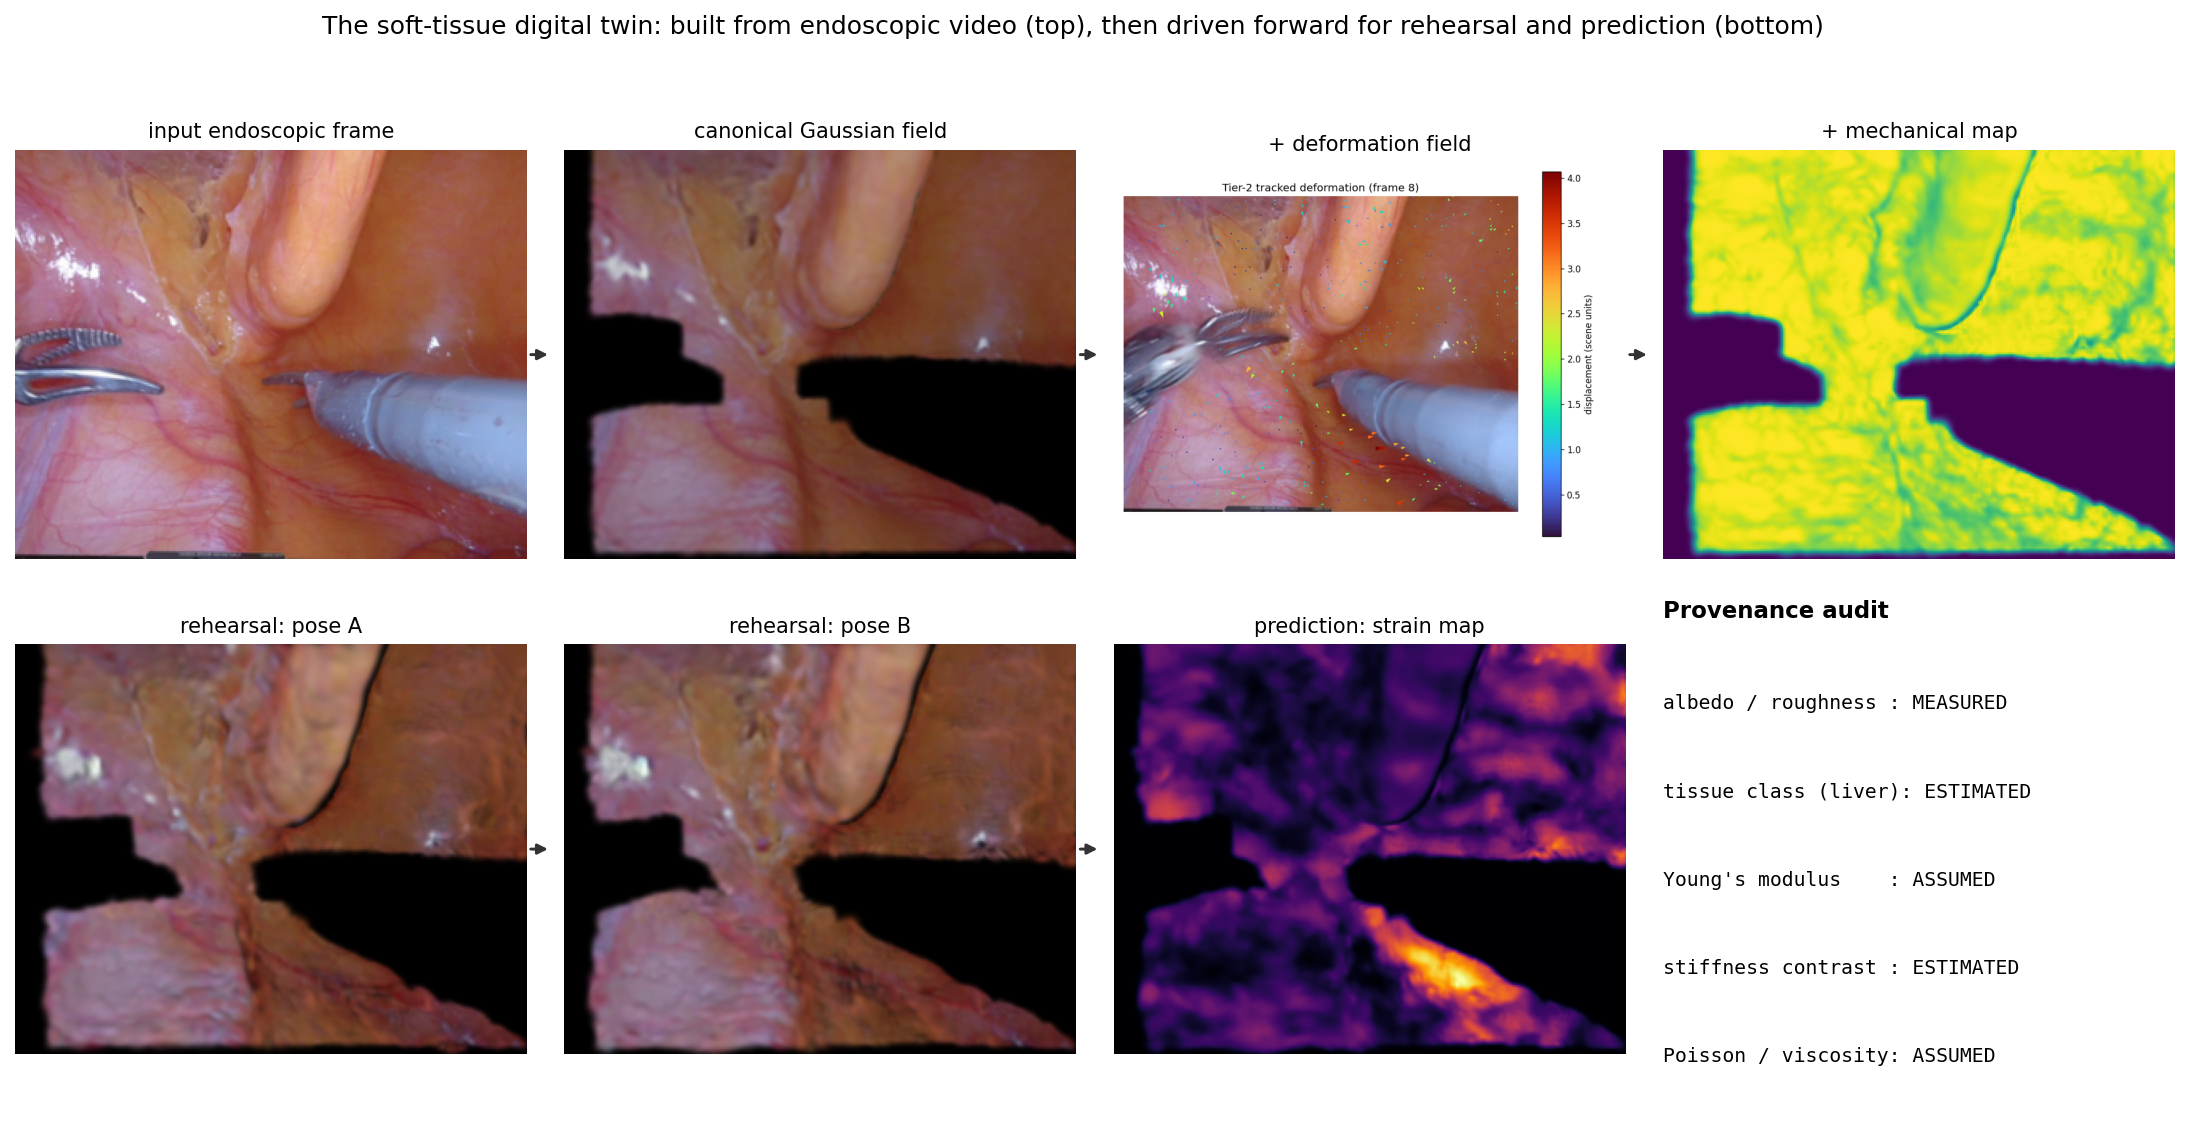
\includegraphics[width=\textwidth]{fig_twin_complete.png}
\caption{The soft-tissue digital twin, end to end. \emph{Top (building the
twin):} from an input endoscopic frame, the pipeline reconstructs the
canonical Gaussian field, tracks the deformation field on it, and attaches a
mechanical parameter map. \emph{Bottom (using the twin):} the twin is then
driven forward in the simulator to rehearsal poses, produces a strain
prediction, and reports a provenance audit that tags every parameter as
measured, estimated, or assumed. This is the complete input$\to$twin$\to$output
result that the subsequent sections break down stage by stage.}
\label{fig:twin_complete}
\end{figure*}

\subsection{Canonical scene reconstruction}
\begin{table}[htbp]
\centering
\caption{Reconstruction (tissue-masked PSNR).}
\label{tab:tier1}
\footnotesize
\begin{tabular}{lcccc}
\toprule
Scene & Frames used & Tissue coverage & Gaussians & Tissue PSNR (dB) \\
\midrule
EndoNeRF pulling & 16--24 & 70.7\% & 6498 & \textbf{36.79} \\
EndoNeRF cutting & 16--24 & 74.1\% & 6824 & \textbf{34.09} \\
SCARED keyframe\_1 & 1 & 78.4\% & 7221 & 26.99 \\
SCARED keyframe\_2 & 1 & 83.1\% & 7676 & 26.17 \\
\bottomrule
\end{tabular}
\end{table}

\begin{table}[htbp]
\centering
\caption{Reconstruction comparison (PSNR in dB). Literature numbers use a
different protocol (held-out novel views, full image) and are indicative;
ours are canonical-field tissue-masked fits.}
\label{tab:recon_compare}
\small
\begin{tabular}{lcc}
\toprule
Method & Protocol & PSNR (dB) \\
\midrule
EndoNeRF \citep{endonerf} & NVS, held-out views & 37.61 \\
EndoSurf \citep{endosurf} & NVS, held-out views & 37.24 \\
EndoGaussian \citep{endogaussian} & NVS, held-out views & 37.89 \\
Prior work (our NVS line) & NVS, 14-frame train & 24.80 \\
\midrule
\textbf{Ours (pulling)} & canonical, tissue-masked & \textbf{36.79} \\
\textbf{Ours (cutting)} & canonical, tissue-masked & \textbf{34.09} \\
\bottomrule
\end{tabular}
\end{table}

All-image PSNR is lower by design because tools are masked out and not
reconstructed; we report tissue-masked PSNR throughout.
Fig.~\ref{fig:tier1} shows the reconstruction on both EndoNeRF scenes. The
pulling scene reconstructs better than cutting because its tissue occupies
a larger, more uniformly lit fraction of the frame and its deformation is
slower. The dominant error in both scenes is at the tool--tissue boundary.
The SCARED result is lower because it uses a single view per keyframe with
moving-camera stereo and no multi-frame supervision, but it confirms
portability across anatomy, camera, and metric scale
(Fig.~\ref{fig:tier1}).

\begin{figure}[htbp]
\centering
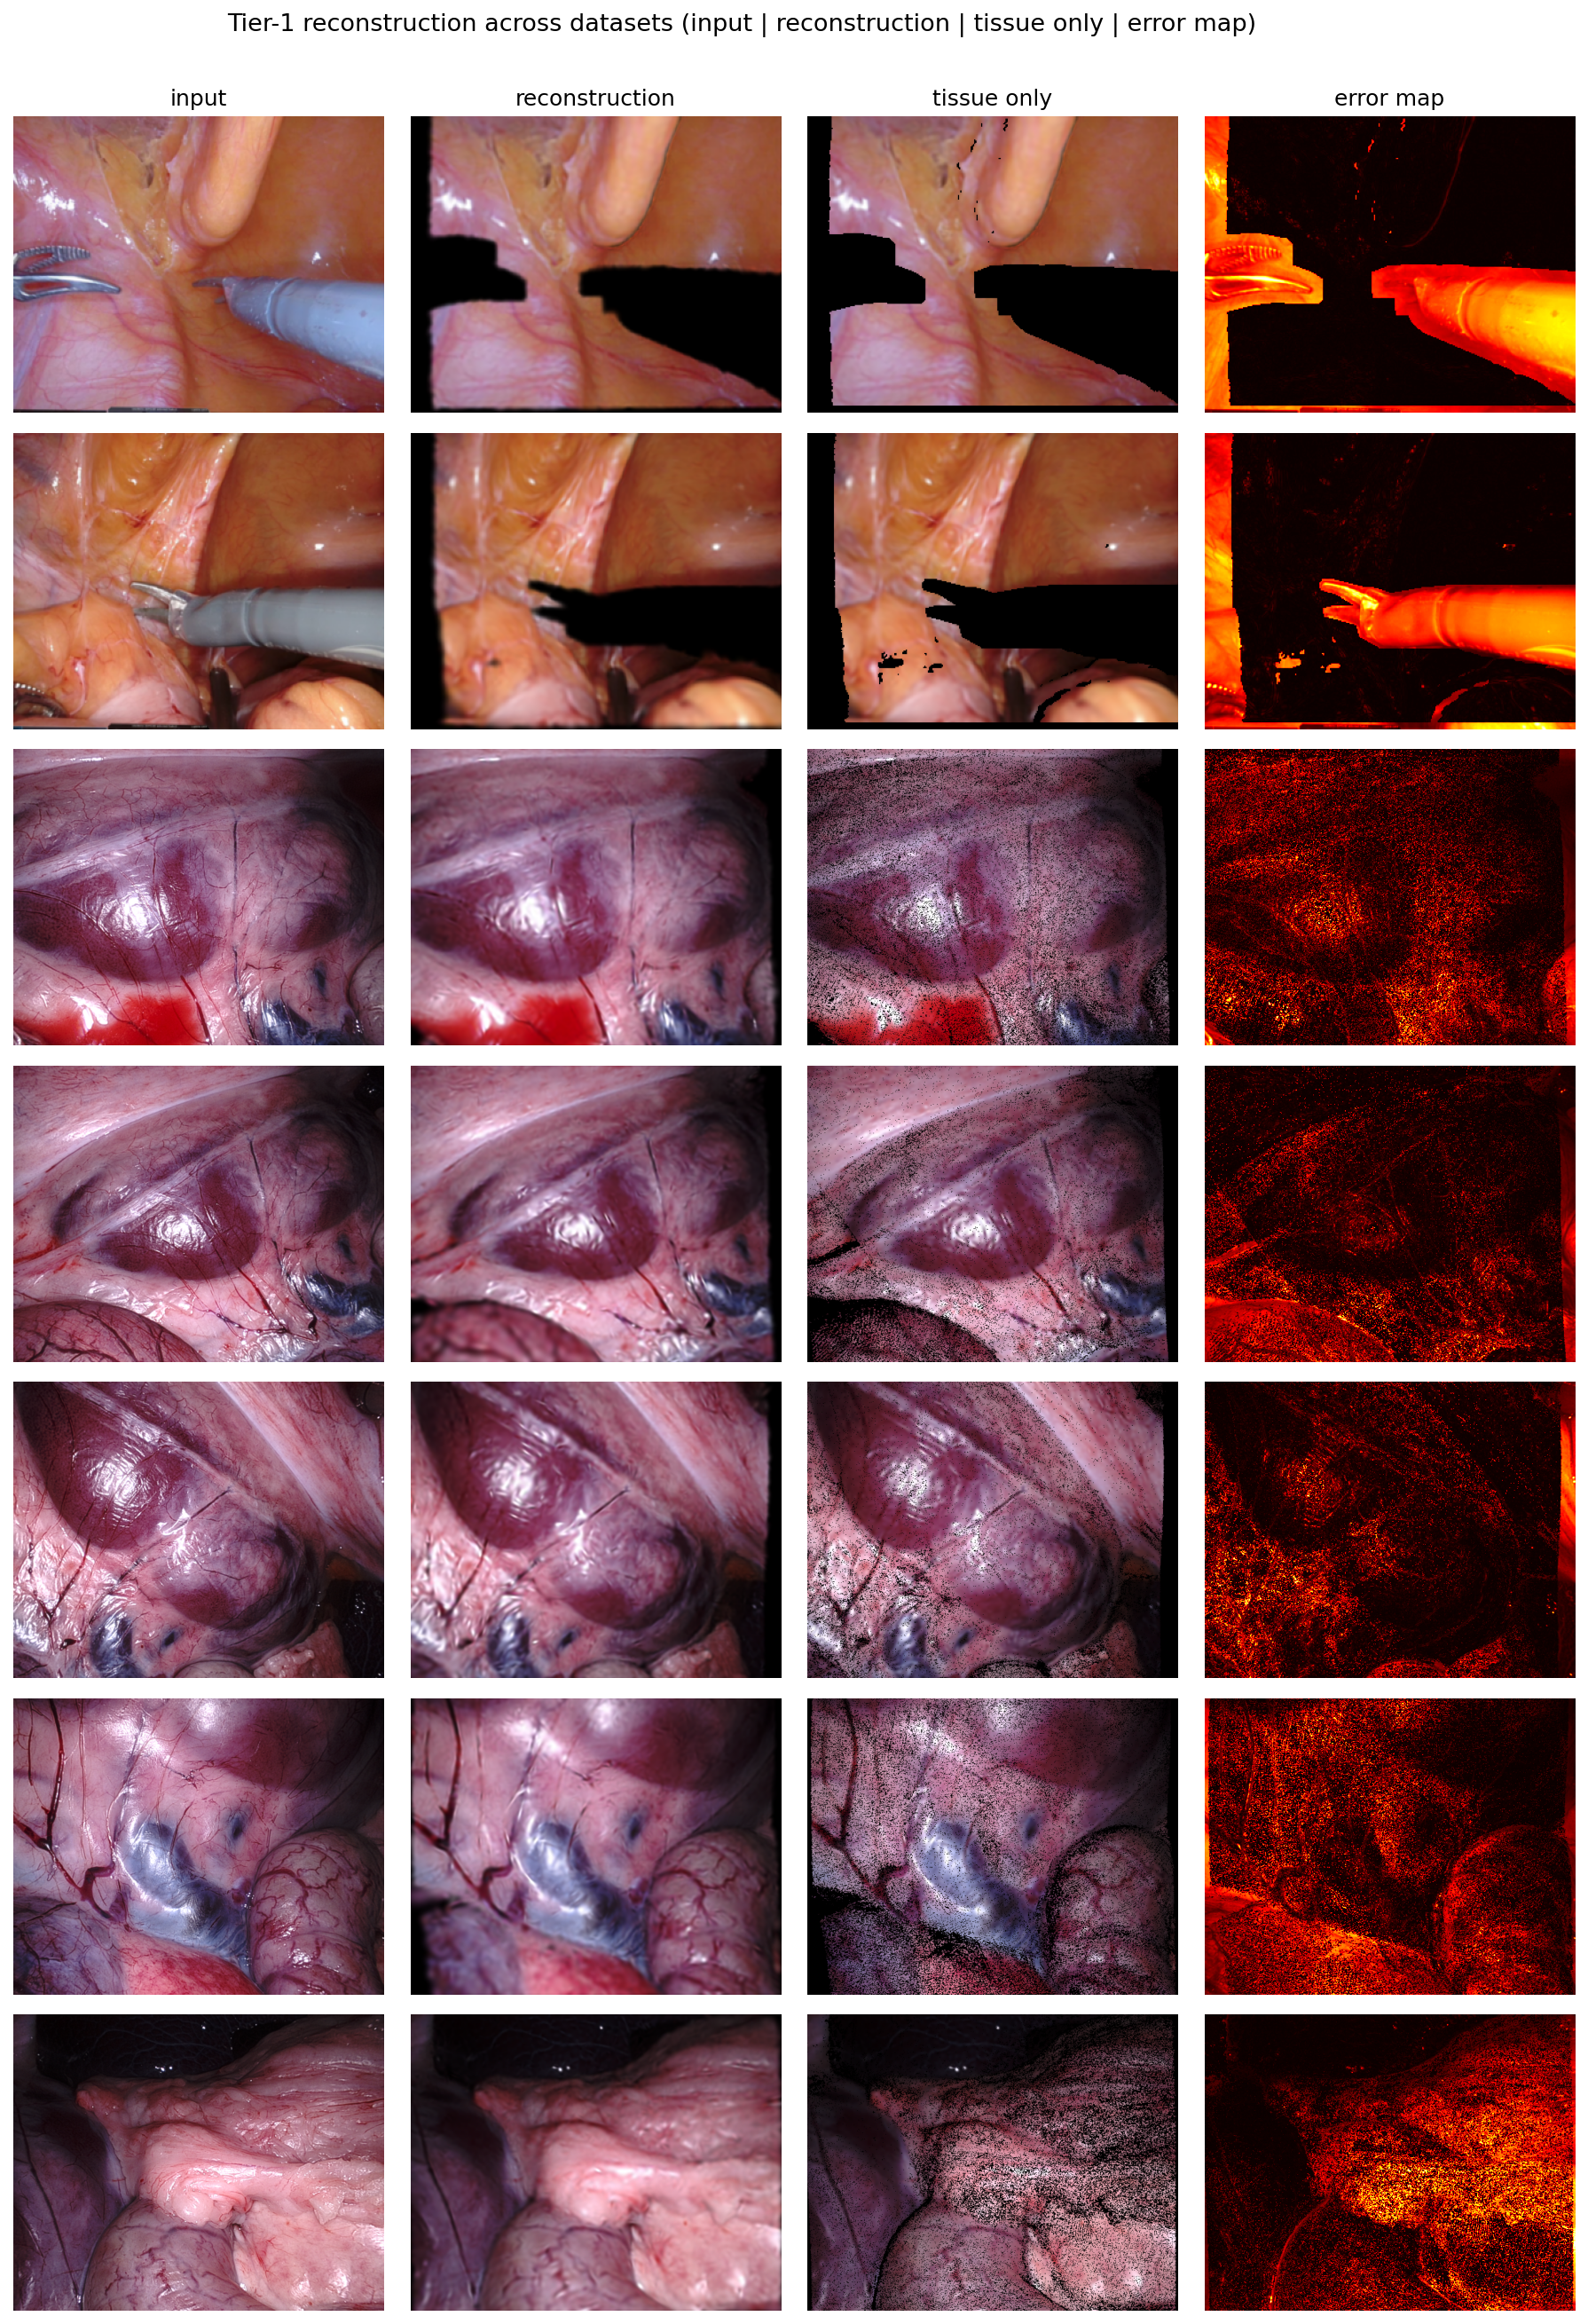
\includegraphics[width=\linewidth]{fig_recon_grid.png}
\caption{Reconstruction across seven datasets/views (rows: EndoNeRF
pulling, EndoNeRF cutting, and SCARED keyframes 1--5). Columns: input $|$
reconstruction $|$ tissue only $|$ error map, with tissue-masked PSNR
annotated per row. The field reconstructs tissue faithfully on the
endoscopic scenes and transfers to real stereo laparoscopy without
retuning.}
\label{fig:tier1}
\end{figure}

\subsection{Deformation tracking}
\begin{table}[htbp]
\centering
\caption{Temporal-model model ablation (pulling scene).}
\label{tab:tier2}
\small
\begin{tabular}{lcc}
\toprule
Tracker & Worst-frame loss & Behaviour \\
\midrule
Inertia-only & 37.23 & frame 5 divergence \\
Const-vel + rollback & 1.55 & frame 5 rolled back \\
\bottomrule
\end{tabular}
\end{table}

Fig.~\ref{fig:tier2} shows the tracked deformation field; displacement
concentrates at the tool contact region. The inertia-only baseline fails on
frame 5 of the pulling scene because that frame contains a fast, partially
occluded retraction in which the photometric gradient is locally
uninformative; the constant-velocity initialization and acceleration prior
track it without divergence, and the rollback prevents a single bad frame
from corrupting the sequence. On the cutting scene the same tracker runs
six frames without divergence (loss 0.52--0.71).

\begin{figure}[htbp]
\centering
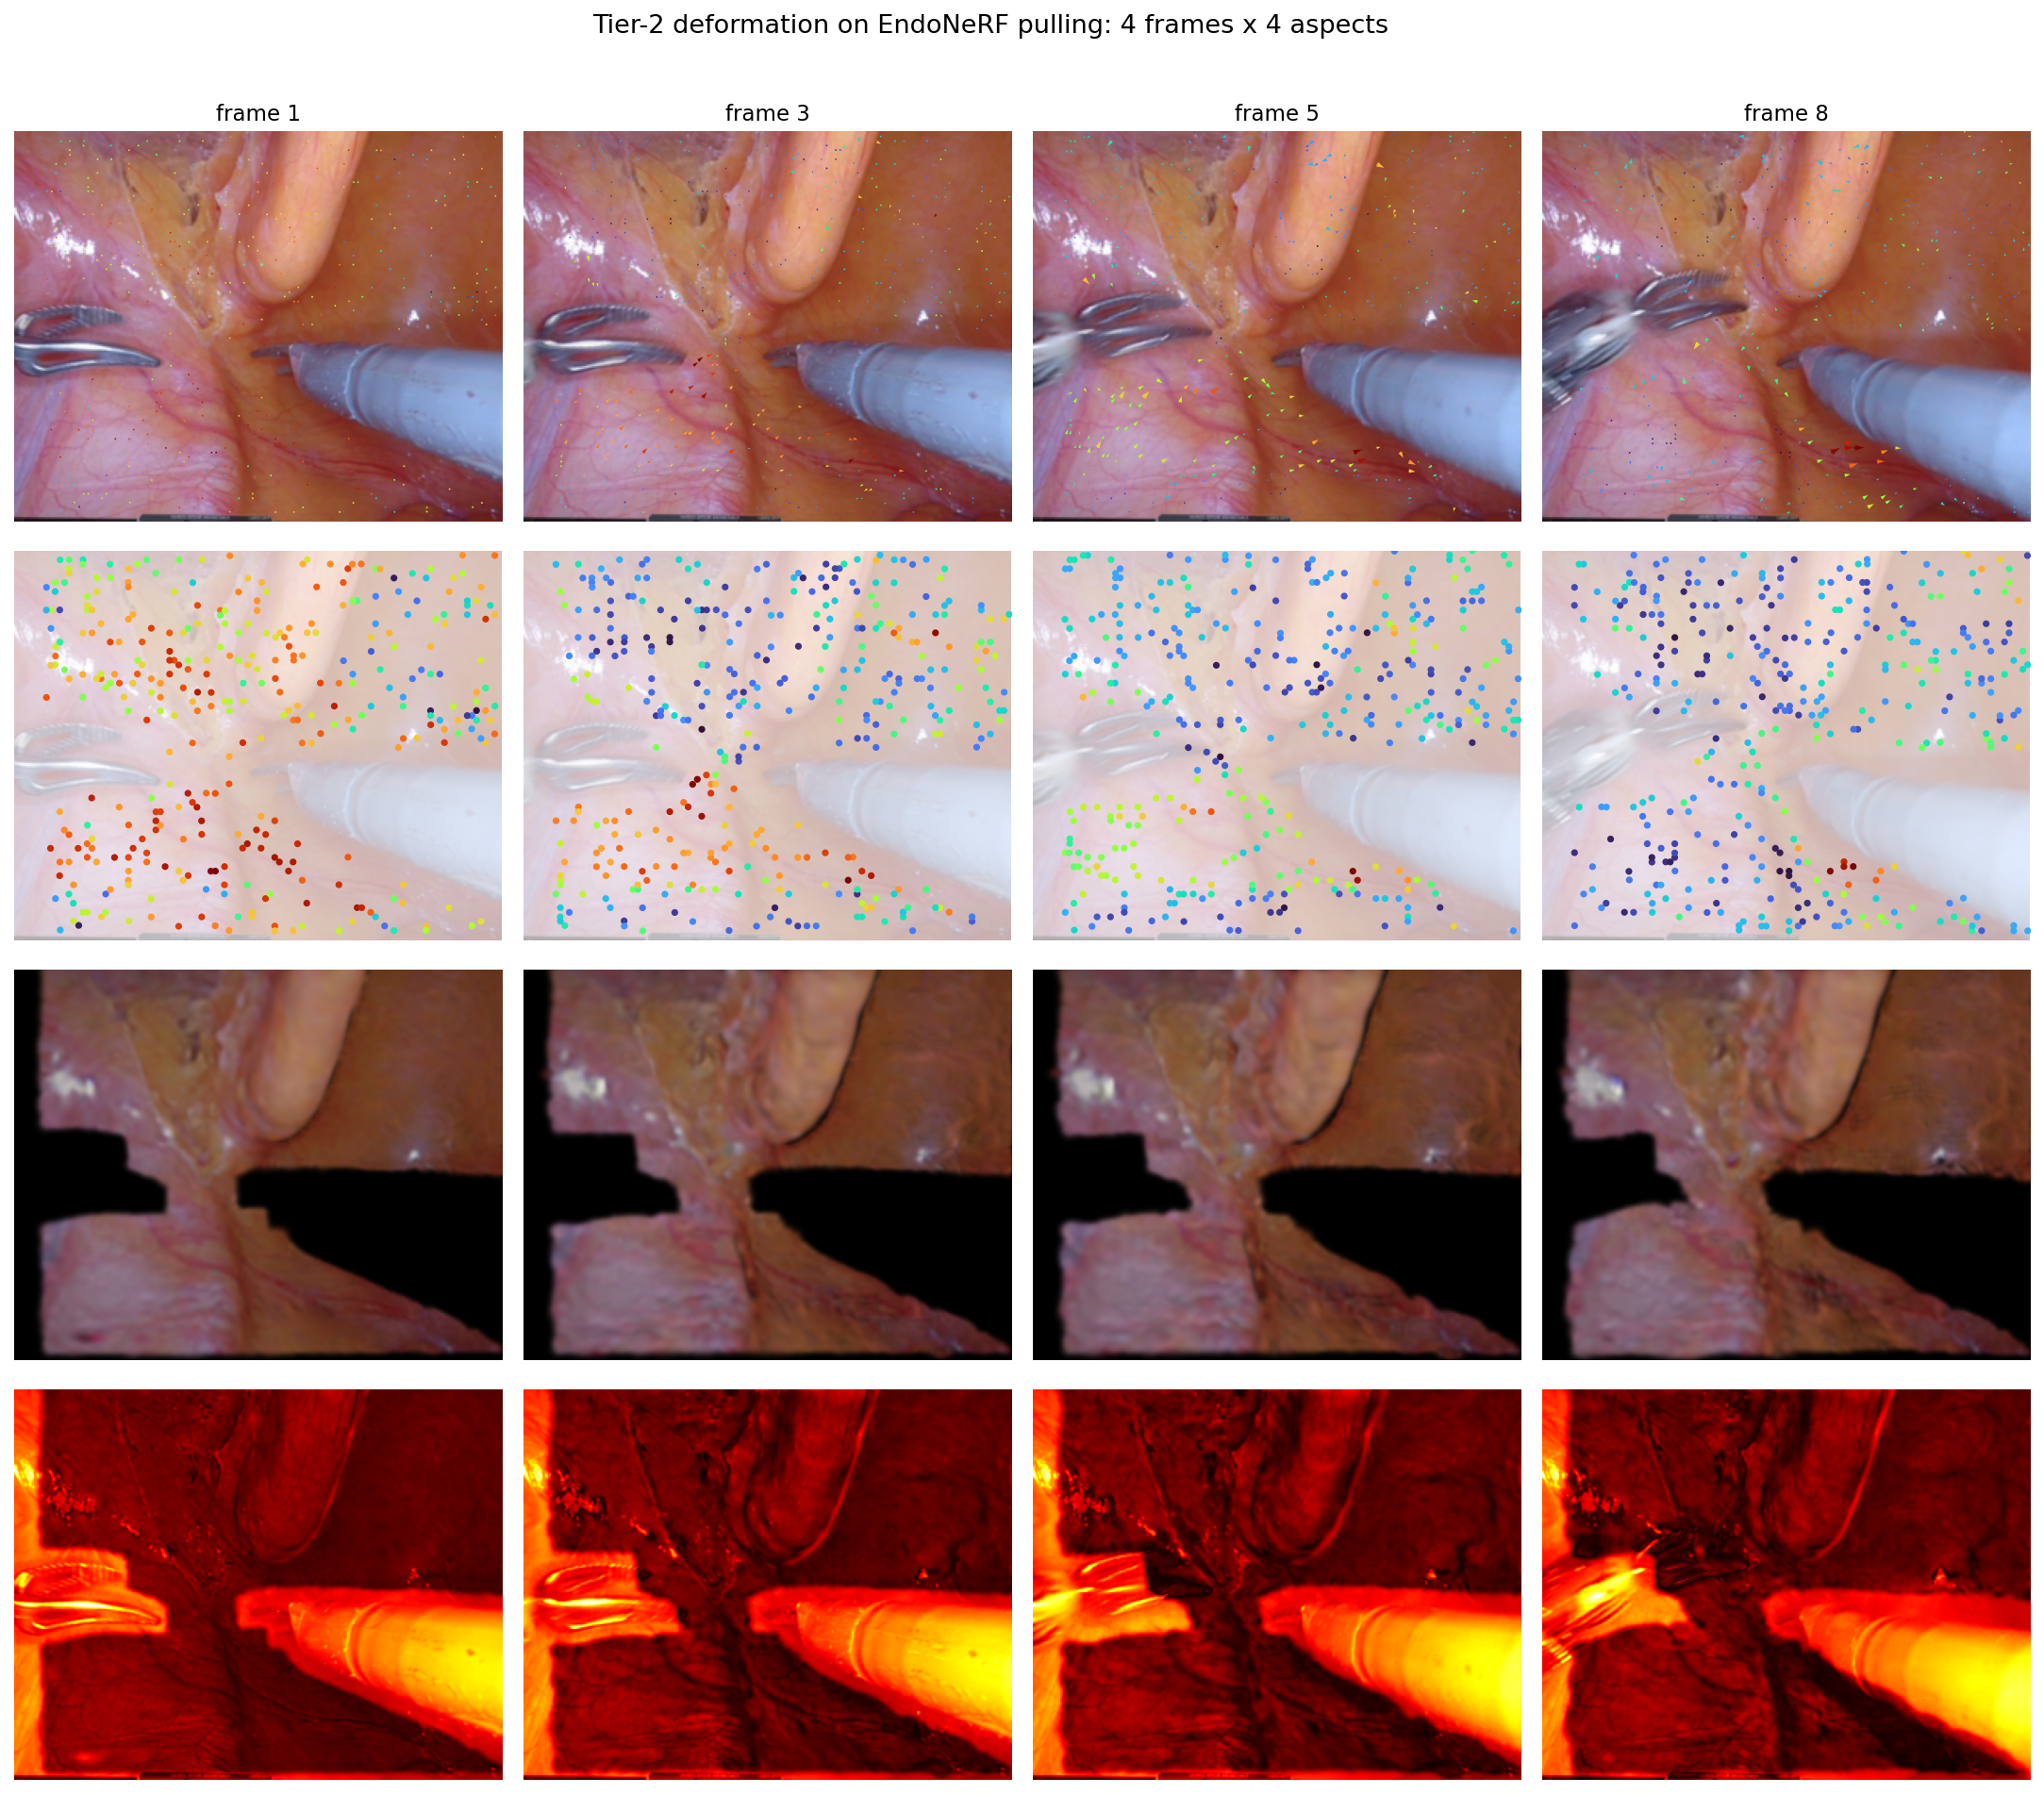
\includegraphics[width=\linewidth]{fig_deform_4x4.png}
\caption{Deformation on EndoNeRF pulling, four frames (columns)
$\times$ four aspects (rows): quiver overlay, displacement-magnitude
heatmap, deformed-field render, and photometric error map. The tracked
displacement grows and localizes at the tool contact, and the deformed
render matches the observed frame.}
\label{fig:tier2}
\end{figure}

\subsection{Mechanical parameter inversion}
Table~\ref{tab:ladder} summarizes the four-stage validation.

\begin{table*}[htbp]
\centering
\caption{Mechanical-inversion staged validation. The four main stages are
the synthetic closed loop, the independent FEM benchmark, the
force-provenance study, and the real phantom; the remaining rows are
sub-experiments of the FEM stage.}
\label{tab:ladder}
\small
\begin{tabular}{@{}p{0.27\linewidth}p{0.32\linewidth}p{0.29\linewidth}@{}}
\toprule
Stage & Evidence & Result \\
\midrule
Synthetic closed loop (mass--spring) & uniform $E$ & 0.01\% error \\
Synthetic inclusion (mass--spring) & $4.0\times$ contrast, surface-only & $3.19\times$ \\
Independent FEM benchmark & $E_{bg}$, measured force + noise & \textbf{median 4.3\% error (6 scen.)} \\
Held-out load case (FEM) & press\_left $\rightarrow$ other cases & within 4.1\% of oracle \\
Noise robustness (FEM) & +0.5 / +1.0\,mm noise & $E_{bg}$ err 13--20\% / 9--23\% \\
Surrogate cross-check & mass--spring vs FEM & 82\% error $\Rightarrow$ FEM needed \\
UQ honesty & Laplace posterior & inclusion flagged unidentified \\
Force provenance & video-force error $\rightarrow$ $E$ & $E_{bg}$ 4.1$\pm$4.0\%; contrast immune \\
\textbf{Real phantom (\'ETS)} & contrast vs Bose truth & \textbf{6.9\% error, CI covers truth} \\
\bottomrule
\end{tabular}
\end{table*}

\paragraph{Synthetic closed loop}
Uniform modulus is recovered to 0.01\% error; a $4\times$ stiff inclusion
is recovered at $3.19\times$ contrast from surface-only observations with
two load cases (Fig.~\ref{fig:tier3}).

\begin{figure}[htbp]
\centering
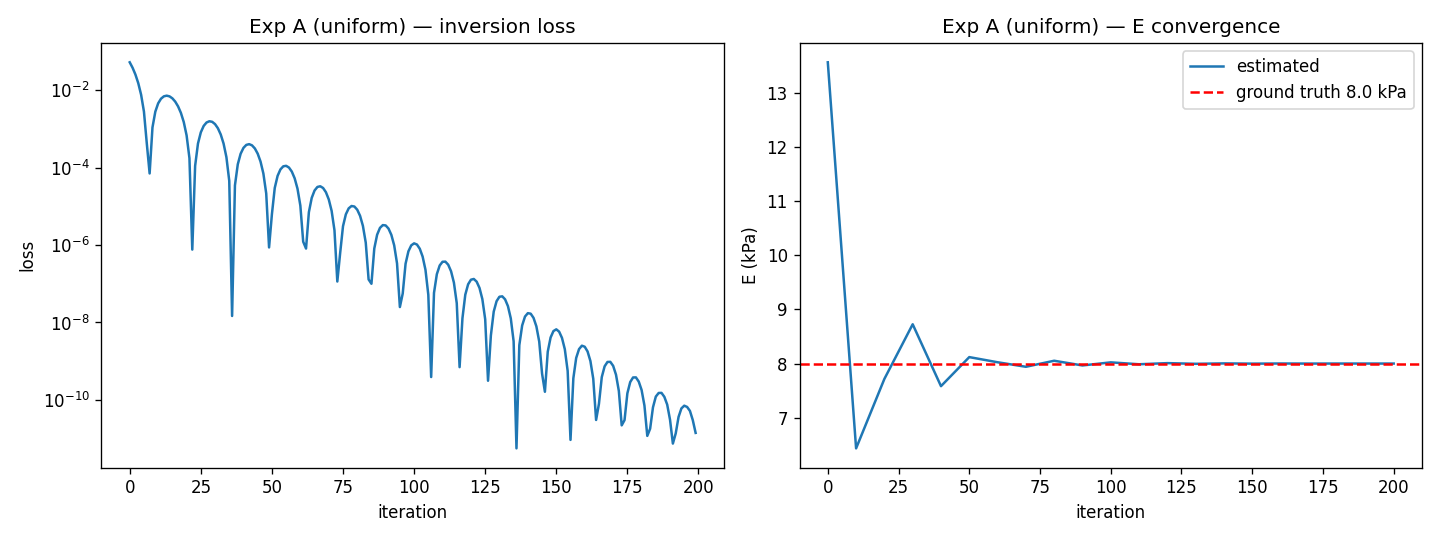
\includegraphics[width=0.49\linewidth]{fig_tier3_uniform.png}
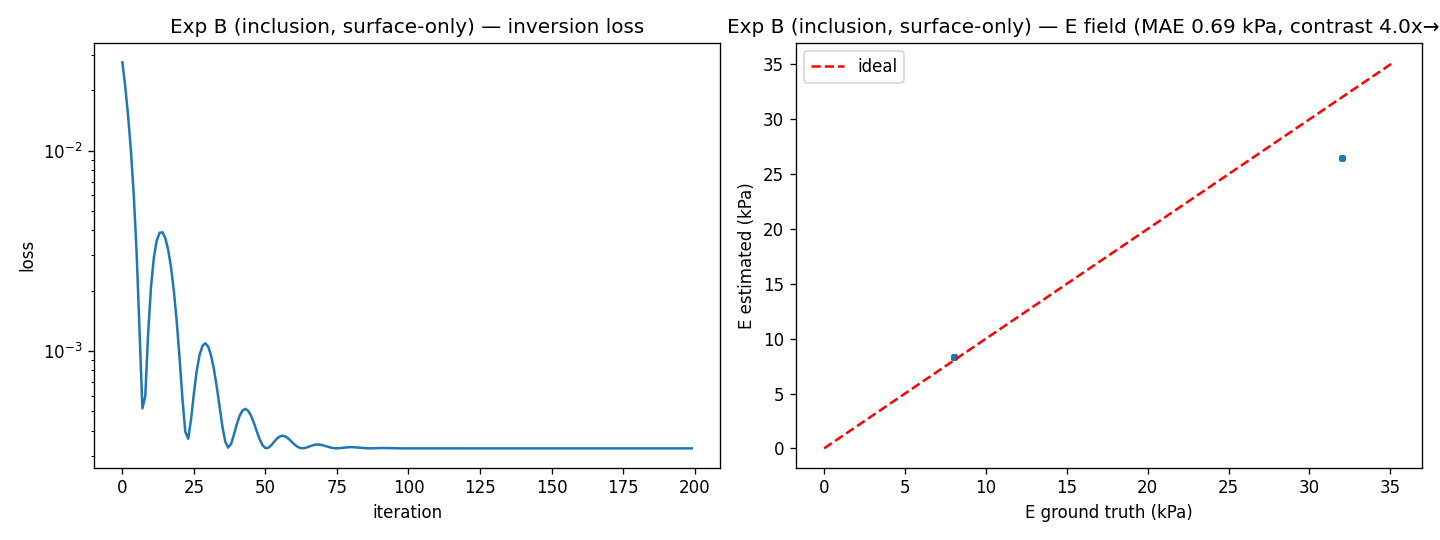
\includegraphics[width=0.49\linewidth]{fig_tier3_inclusion.png}
\caption{Synthetic closed loop: (left) uniform $E$ converges to the
8.0\,kPa ground truth; (right) stiff-inclusion contrast $4.0\times$ $\to$
$3.19\times$.}
\label{fig:tier3}
\end{figure}

\paragraph{Independent FEM benchmark}
With measured forces (5\% calibrated error) and noisy surface motion, the
background modulus is recovered to a median error of 4.3\% (mean 9.4\%)
across six scenarios (per-scenario values in
Table~\ref{tab:perscenario}). Accuracy is regime-dependent: it is below 6\%
on stiff backgrounds ($E_{bg} \ge 3.8$\,kPa) but reaches 17--27\% on the
two softest ($E_{bg} \approx 2.6$\,kPa), where the small absolute
displacements degrade the signal-to-noise ratio of the deformation
observation. The inclusion contrast is recovered to a mean of $1.90\times$
against a ground-truth mean of $2.41\times$. Material inverted on
\texttt{press\_left} predicts unseen load cases with displacement error
11.1\% (\texttt{press\_right}), 3.7\% (\texttt{shear\_x}), and 14.9\%
(\texttt{shear\_y}), against oracle-material errors of 9.6\%, 7.2\%, and
10.9\% respectively (Fig.~\ref{fig:fem_perscenario} and
Fig.~\ref{fig:fem_dist}).

\begin{table}[htbp]
\centering
\caption{Per-scenario FEM-benchmark background-modulus inversion.}
\label{tab:perscenario}
\small
\begin{tabular}{lcccc}
\toprule
Scenario & $E_{bg}^{gt}$ (kPa) & $E_{bg}^{est}$ (kPa) & Error (\%) & Contrast est/gt \\
\midrule
000 & 7.35 & 7.24 & 1.6 & $2.26\times / 1.71\times$ \\
001 & 2.61 & 2.17 & 17.1 & $2.09\times / 2.79\times$ \\
002 & 3.81 & 3.90 & 2.3 & $1.34\times / 3.66\times$ \\
003 & 7.78 & 7.54 & 3.1 & $1.30\times / 1.00\times$ \\
004 & 2.81 & 2.05 & 26.9 & $2.00\times / 1.30\times$ \\
005 & 4.57 & 4.82 & 5.5 & $2.38\times / 3.99\times$ \\
\midrule
\multicolumn{3}{l}{median / mean error} & 4.3 / 9.4 & mean $1.90\times / 2.41\times$ \\
\bottomrule
\end{tabular}
\end{table}

\begin{figure}[htbp]
\centering
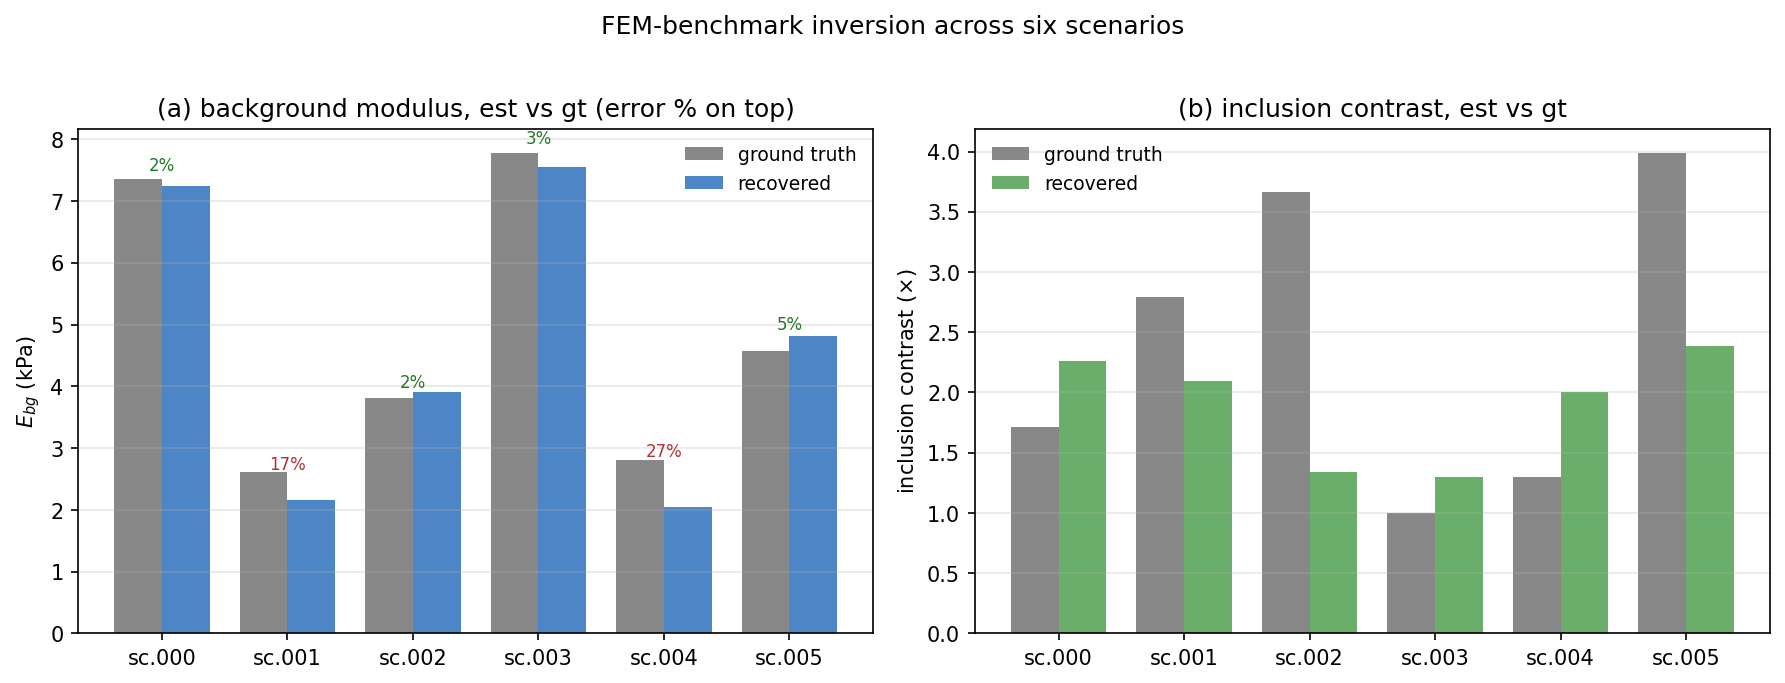
\includegraphics[width=\linewidth]{fig_fem_perscenario.png}
\caption{Per-scenario FEM-benchmark inversion. (a) Background modulus,
recovered vs ground truth, with the relative error annotated (green $<10\%$,
red $>10\%$). (b) Inclusion contrast, recovered vs ground truth. The two
softest backgrounds (sc.\ 001, 004) are the hardest, consistent with the
regime-dependence analysis.}
\label{fig:fem_perscenario}
\end{figure}

\begin{figure}[htbp]
\centering
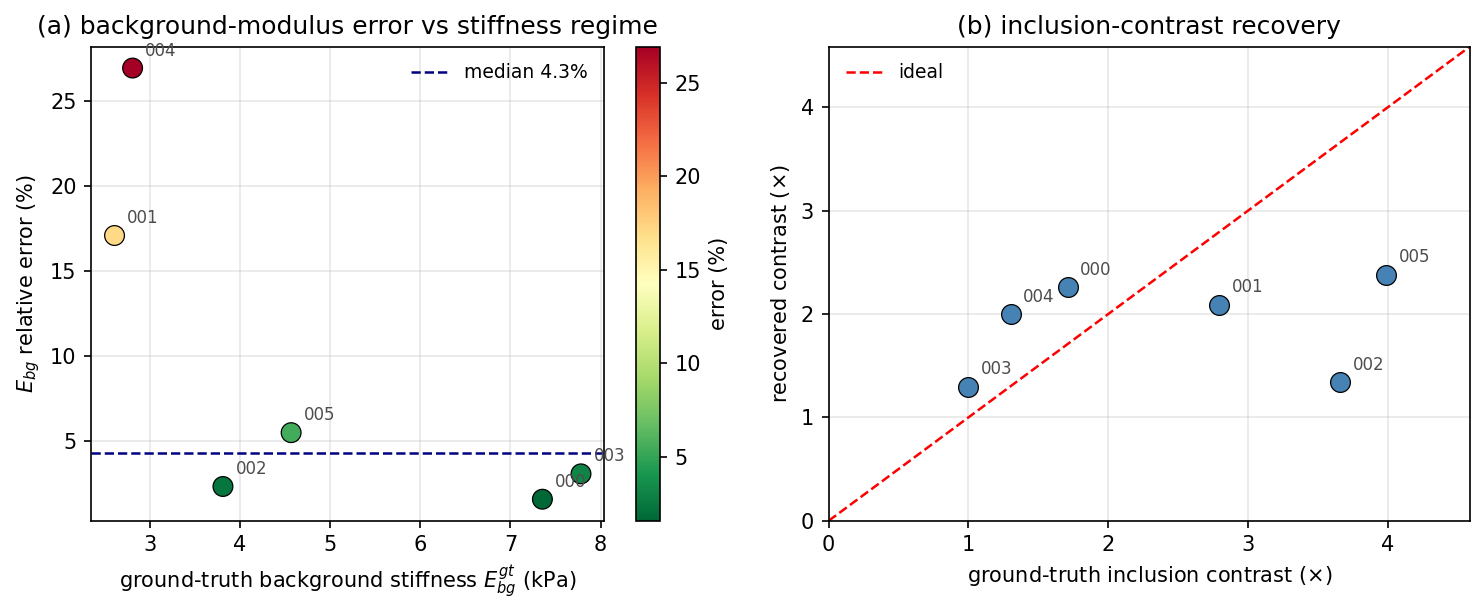
\includegraphics[width=0.85\linewidth]{fig_fem_distribution.png}
\caption{FEM-benchmark inversion across six scenarios. (a) Background-modulus
error vs ground-truth stiffness: accuracy is regime-dependent, degrading on
the two softest backgrounds. (b) Recovered inclusion contrast vs ground
truth (dashed identity).}
\label{fig:fem_dist}
\end{figure}

\paragraph{Force provenance}
\label{sec:force}
We extract the empirical error model of a real video-based force estimator
(small-bowel retraction benchmark, 3D-ResNet, 6373 samples / 50 recordings:
MAE 0.295\,N, systematic scale factor $0.949 \pm 0.140$)
\citep{smallbowelforce} and transport it onto the FEM benchmark. A
systematic sweep (force scale 0.80--1.20 $\to$ $E_{bg}$ ratio
0.846--1.110) confirms the one-to-one force-to-modulus propagation of
Proposition~\ref{prop:forcescale}. With the full empirical model, the
$E_{bg}$ error is 4.1\,$\pm$\,4.0\% and the stiffness contrast stays
2.22--2.27$\times$ regardless of force error, consistent with the
scale-invariance of the contrast ratio.

\paragraph{Real phantom}
On the \'ETS indentation phantom (6 acquisitions), the image-derived
modulus contrast reaches a median of $3.80\times$ (bootstrap 95\% CI
[3.16, 4.34]) against compression-test truth $3.56\times$ (background
$31.0 \pm 1.87$\,kPa, inclusion $8.71 \pm 3.80$\,kPa), a 6.9\% relative
error, stable across 9 sensitivity configurations (3.5--9.3\%). Posterior
intervals contain both ground-truth moduli. The estimate is a contrast, not
an absolute modulus, and Proposition~\ref{prop:forcescale} explains why
this ratio is the trustworthy quantity; the posterior intervals are
calibrated, containing both ground-truth moduli.
Fig.~\ref{fig:ets} shows the per-acquisition estimates.

\begin{figure}[htbp]
\centering
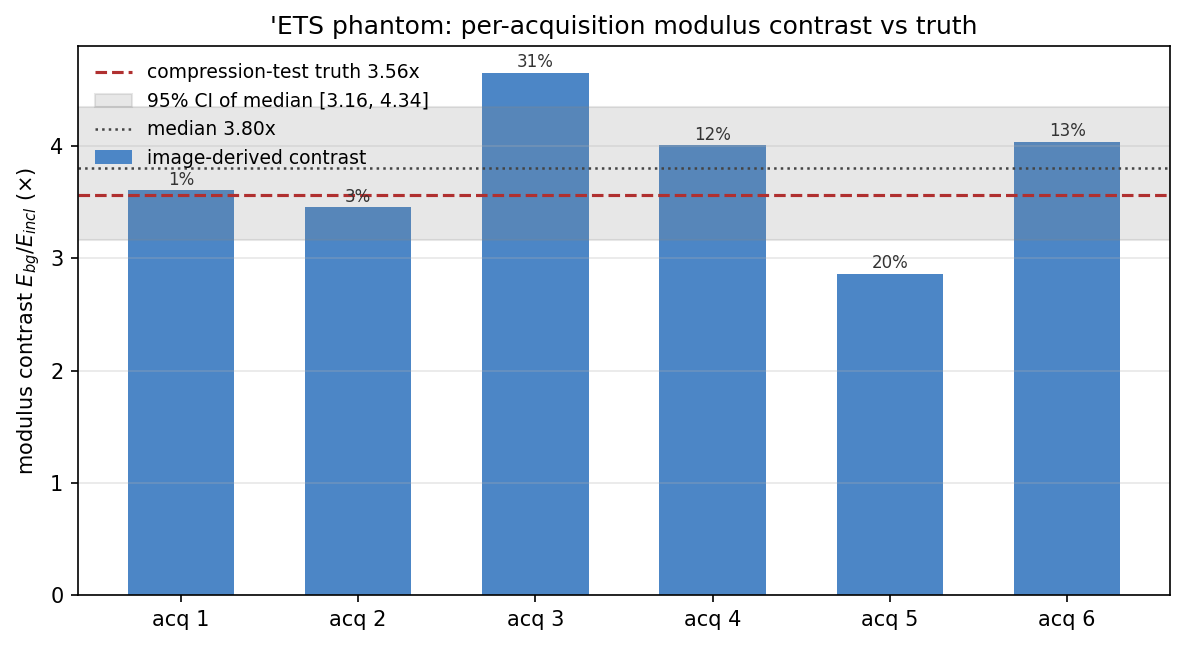
\includegraphics[width=0.7\linewidth]{fig_ets.png}
\caption{\'ETS phantom: per-acquisition image-derived modulus contrast vs
the compression-test truth (dashed), with the bootstrap 95\% CI band and
median. The video-derived contrast is consistent across all six
acquisitions.}
\label{fig:ets}
\end{figure}

\paragraph{Hospital CT validation}
To validate the tissue classification on independent clinical data, we
reconstruct the liver from an abdominal CT scan of a patient from Henan
Provincial People's Hospital (Fig.~\ref{fig:hospital_ct}). A
right-upper-quadrant liver region is segmented on 82 axial slices and
meshed into a patient-specific liver geometry (178k vertices). The CT
confirms the anatomy is liver, which is consistent with the optical tissue
classification produced by the twin's classifier on endoscopic video
(liver). The CT-derived mesh is a patient-specific geometry source for the
twin; the absolute volume is not reported because the slices carry no
spacing metadata.

\begin{figure}[htbp]
\centering
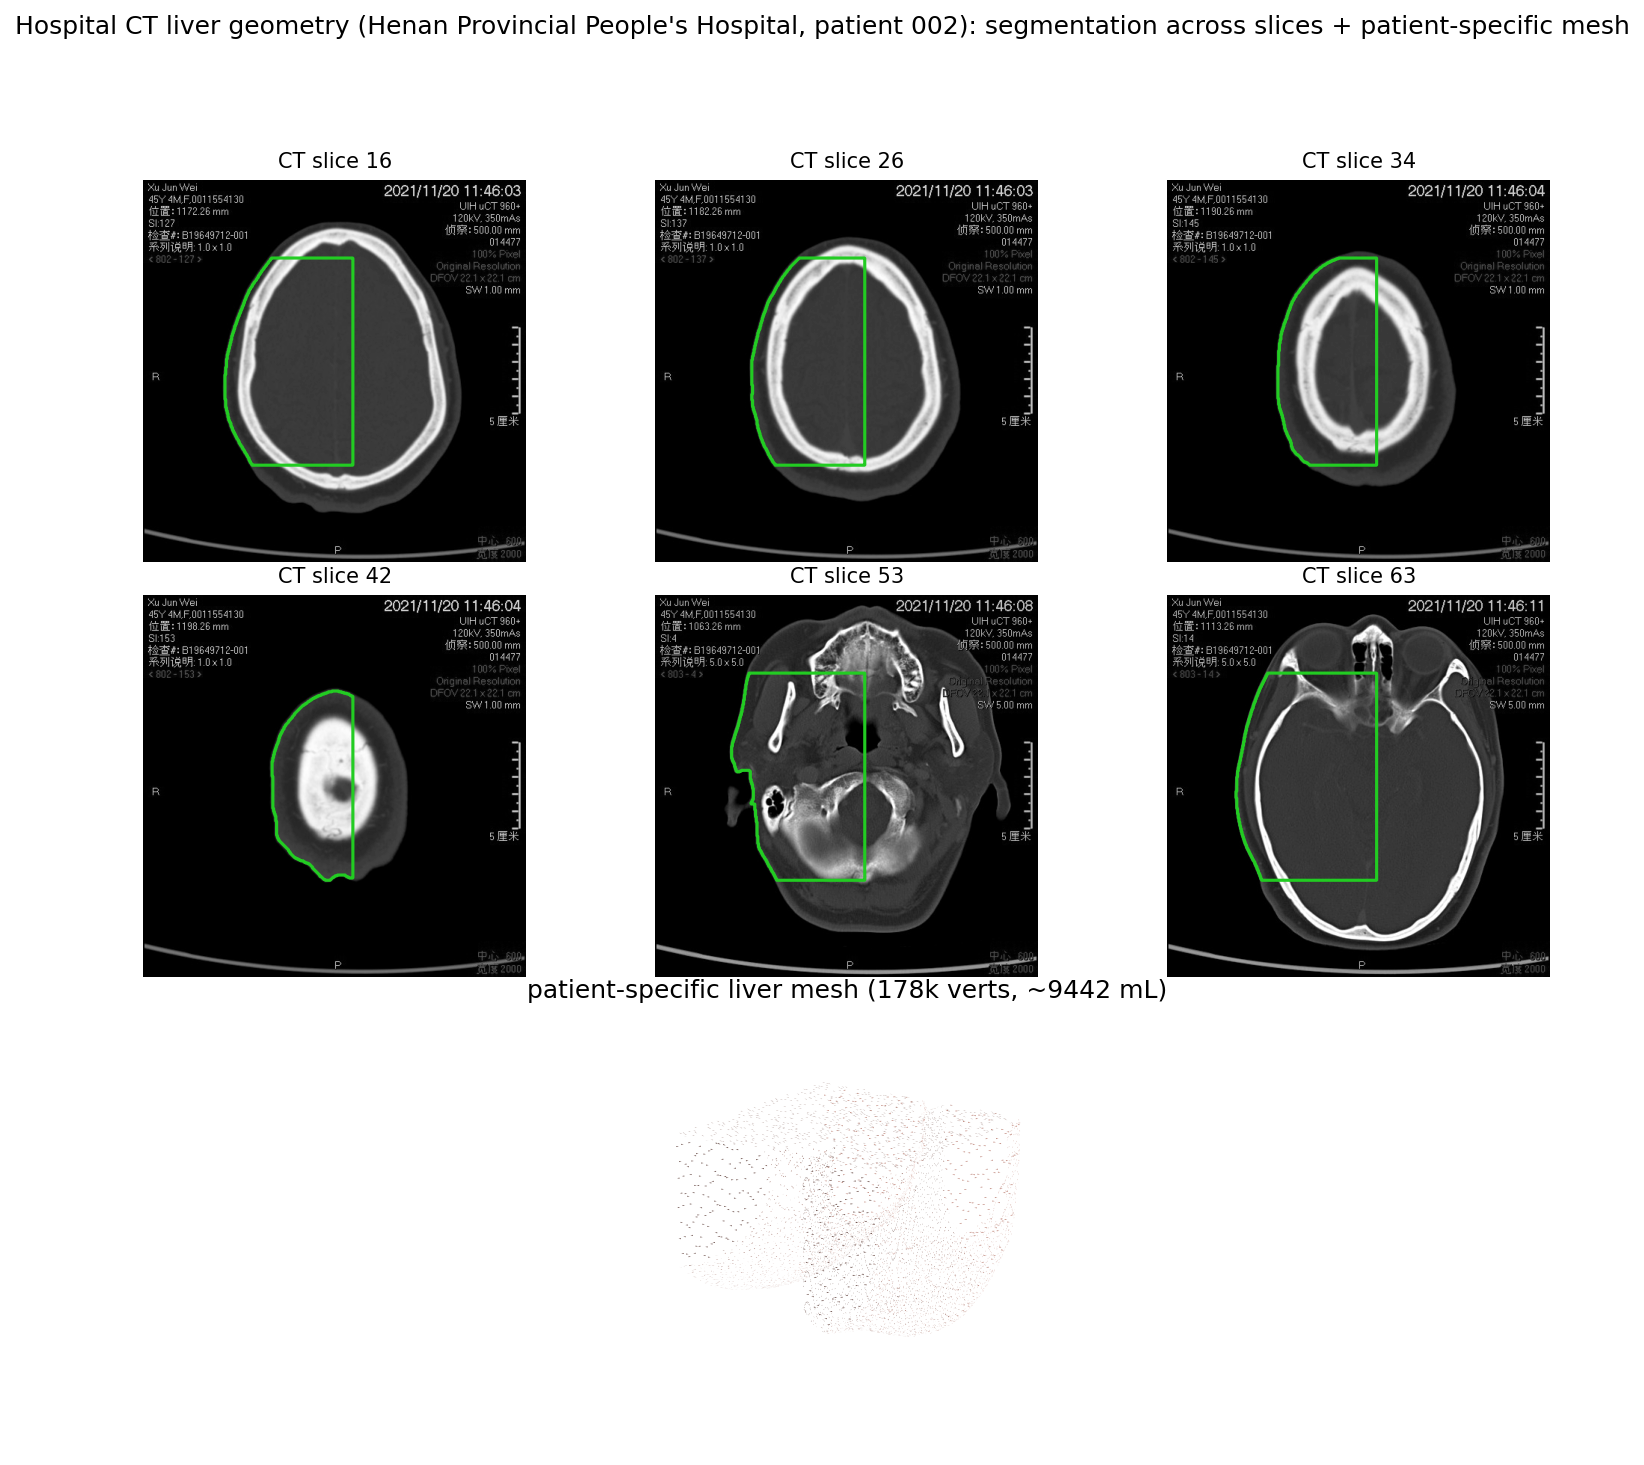
\includegraphics[width=\linewidth]{fig_hospital_ct.png}
\caption{Hospital CT liver geometry (Henan Provincial People's Hospital).
Left: three axial CT slices with the segmented liver region (green).
Right: the patient-specific liver mesh reconstructed from the
segmentation. The CT-confirmed liver anatomy is consistent with the twin's
optical tissue classification (liver).}
\label{fig:hospital_ct}
\end{figure}

\begin{figure}[htbp]
\centering
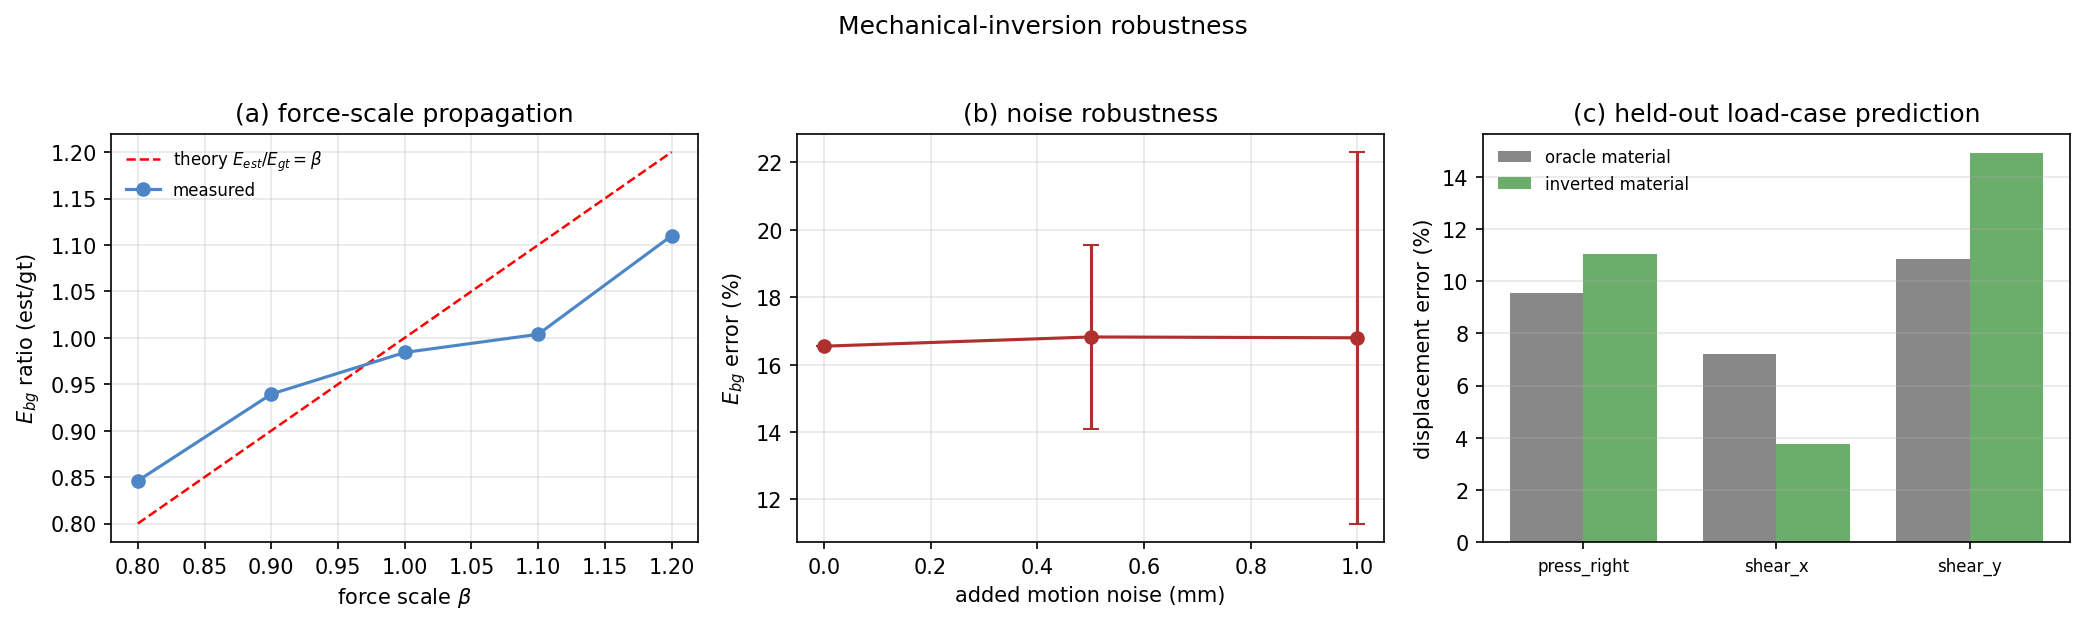
\includegraphics[width=\linewidth]{fig_robustness.png}
\caption{Mechanical-inversion robustness. (a) Force-scale sweep: the
recovered $E_{bg}$ ratio tracks the theoretical one-to-one propagation of
Proposition~\ref{prop:forcescale}. (b) Noise robustness: the $E_{bg}$ error
grows gracefully with added motion noise. (c) Held-out load-case
prediction: the inverted material matches the oracle material across three
unseen load cases.}
\label{fig:robustness}
\end{figure}

\paragraph{Mechanics comparison}
Table~\ref{tab:mech_compare} places the mechanical results against the
closest settings in the literature and our own ablations. Because the
settings differ (known force vs.\ force-free, absolute modulus vs.\
contrast), the comparison is by setting, not by a single leaderboard
number; the consistent observation is that the audit reports the quantity
each setting can support.

\begin{table*}[htbp]
\centering
\caption{Mechanics comparison by setting. ``Abs.\ $E$'' is absolute-modulus
recovery; ``contrast'' is stiffness-contrast recovery.}
\label{tab:mech_compare}
\small
\begin{tabular}{@{}p{0.20\linewidth}p{0.24\linewidth}p{0.18\linewidth}p{0.24\linewidth}@{}}
\toprule
Method & Setting & Force & Result \\
\midrule
PAC-NeRF \citep{pacnerf} & system ID, multi-view & known & abs.\ $E$, object-dependent \\
PhysDreamer \citep{physdreamer} & video prior, static & none & relative stiffness only \\
PhysGaussian \citep{physgaussian} & MPM dynamics & manual $E$ & parameters assigned \\
Prior TMI-line (our group) & image + force joint inv. & measured & abs.\ $E$ err 21--30\% (60 scen.) \\
\midrule
Ours (synthetic closed loop) & uniform $E$ & known & abs.\ $E$ to 0.01\% error \\
Ours (FEM benchmark) & 2-region, surface-only & measured (5\% err) & abs.\ $E_{bg}$ median 4.3\% err \\
Ours (force provenance) & 2-region & video-estimated & $E_{bg}$ 4.1$\pm$4.0\%; contrast invariant \\
Ours (real phantom) & strain ratio & none & contrast 6.9\% err, CI covers truth \\
\bottomrule
\end{tabular}
\end{table*}

\paragraph{Material recovery}
Beyond geometry and motion, the twin recovers the tissue's optical and
mechanical material. Fig.~\ref{fig:material} shows the recovered albedo and
roughness maps from the canonical field (reconstruction) alongside the mechanical
parameters with their audit tags (inversion): the tissue classifies as liver
(Neo-Hookean), and because no force is instrumented, the Young's modulus,
Poisson ratio, density, viscosity, and friction are all honestly tagged
\emph{assumed\_table}, while the optical parameters are \emph{measured}.

\begin{figure}[htbp]
\centering
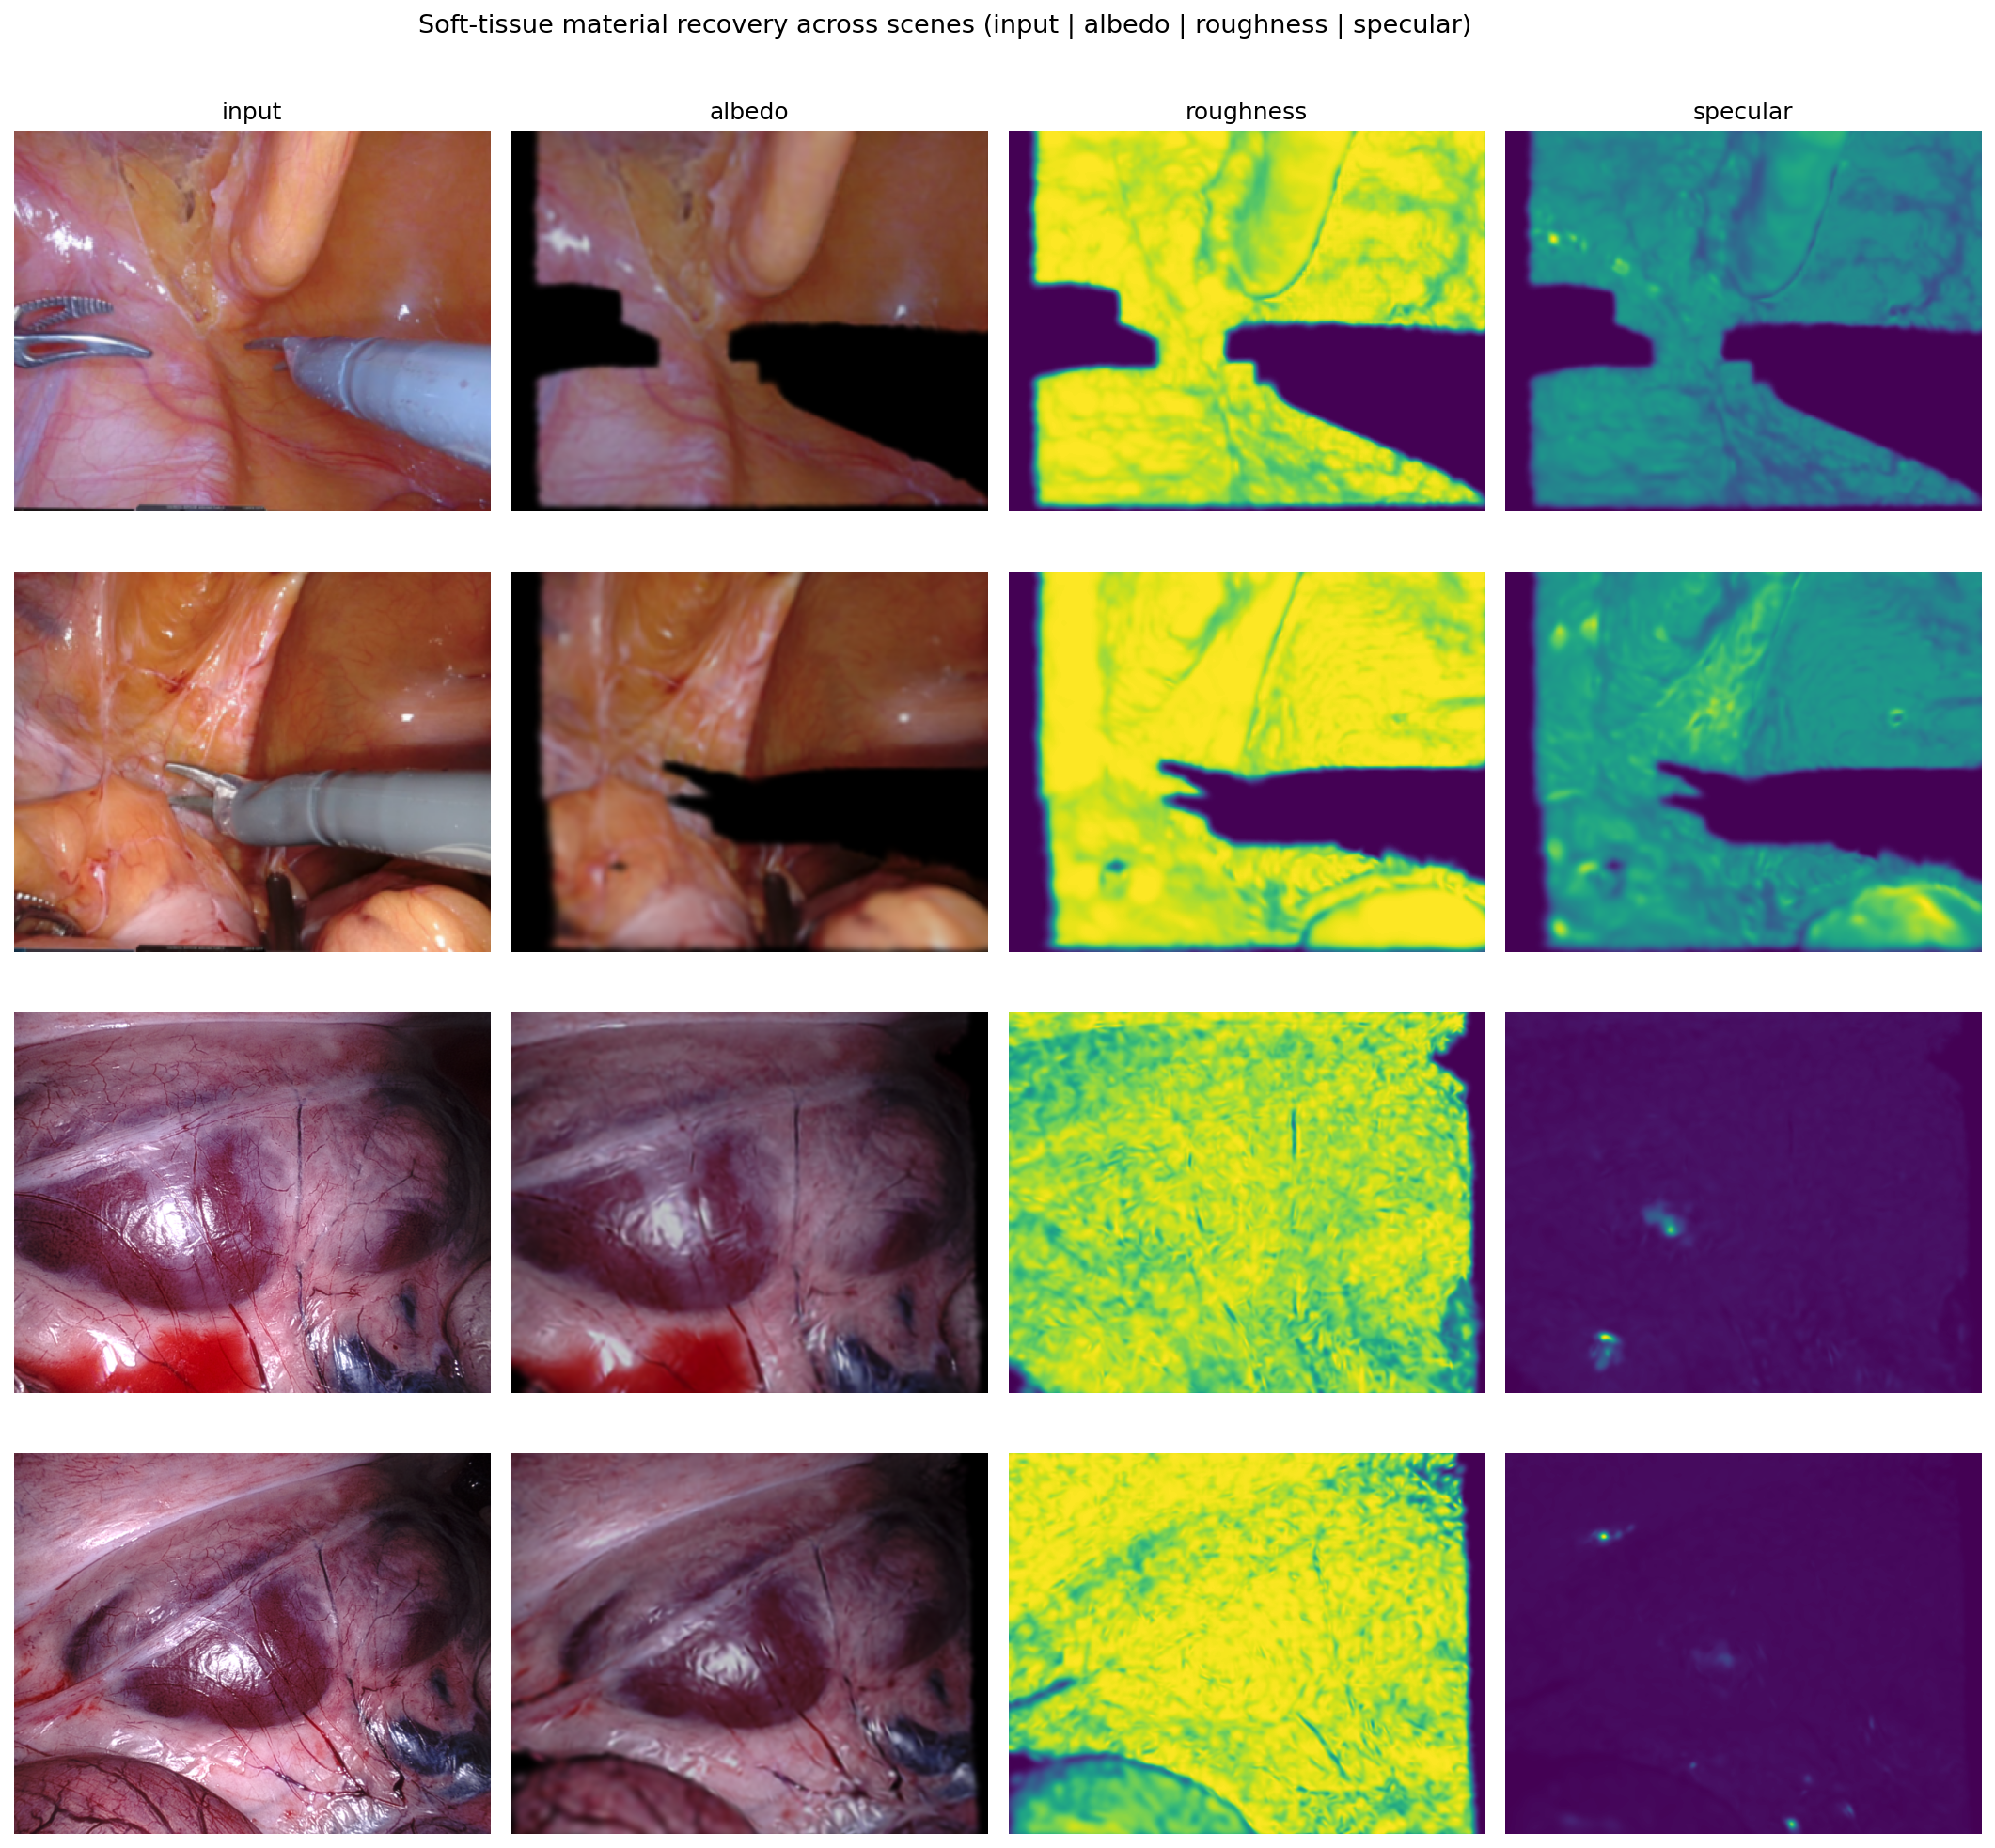
\includegraphics[width=\linewidth]{fig_material_4x4.png}
\caption{Soft-tissue material recovery across four scenes (rows: EndoNeRF
pulling, EndoNeRF cutting, SCARED keyframe\_1, SCARED keyframe\_2).
Columns: input $|$ recovered albedo $|$ recovered roughness $|$ recovered
specular. The optical material is measured; the mechanical parameters are
honestly tagged \emph{assumed} (no force instrumented).}
\label{fig:material}
\end{figure}

\subsection{Uncertainty honesty}
\label{sec:uq_exp}
The Laplace posterior reports a small $\mathrm{std}(\log E_{bg}) = 1.17$
but a much larger $\mathrm{std}(\log E_{incl}) = 21.2$: the data do not
constrain the deep inclusion modulus, consistent with its 30\% estimation
error. The 95\% prediction interval covers 100\% of held-out surface nodes
but is dominated by the unidentified inclusion direction, so the
uncertainty estimate flags the inclusion as unidentifiable rather than
reporting overconfidence.

\subsection{Comparison with related approaches}
\label{sec:comparison}
Table~\ref{tab:position} positions the pipeline against representative
methods. Three distinctions are salient. First, the output is a simulable
twin rather than a reconstruction: EndoNeRF, EndoSurf, and EndoGaussian
produce appearance and geometry but no forward operator $\mathcal{S}$.
Second, the mechanics are recovered rather than assigned: PhysGaussian
requires manually supplied parameters, and PhysDreamer recovers only
relative stiffness, whereas we recover absolute modulus where identifiable
and mark the rest as assumed. Third, the provenance is explicit: no prior
method tags each parameter as measured, estimated, or assumed. The closest
in spirit is PAC-NeRF, which performs system identification with known
forces, but it targets household objects with multi-view capture and does
not audit provenance; our force-provenance study additionally quantifies
how imperfect video-based force estimates bound absolute-modulus accuracy.

\subsection{Component-wise comparison}
\label{sec:componentwise}
Because no prior method builds an audited soft-tissue twin from endoscopic
video, a single end-to-end leaderboard comparison is impossible. We
therefore compare each component against the closest state of the art
(Table~\ref{tab:componentwise}). The reconstruction component is comparable
to the endoscopic novel-view-synthesis methods; the mechanical component is
comparable to the physics-aware system-identification methods; and the
audit component has no direct counterpart.

\begin{table*}[htbp]
\centering
\caption{Component-wise comparison to the closest state of the art.}
\label{tab:componentwise}
\small
\begin{tabular}{@{}p{0.16\linewidth}p{0.24\linewidth}p{0.24\linewidth}p{0.24\linewidth}@{}}
\toprule
Component & Closest SOTA & Their result & Ours \\
\midrule
Reconstruction & EndoGaussian \citep{endogaussian} (NVS) & 37.89\,dB (NVS protocol) & 36.79\,dB (canonical, tissue-masked) \\
 & Prior NVS line (our group) & 24.80\,dB & \textbf{+12\,dB} \\
Deformation tracking & DefSLAM \citep{defslam} & monocular deforming tracking & fixed-topology + rollback, no divergence \\
Mechanics (abs.\ $E$) & PAC-NeRF \citep{pacnerf} & object-dependent, known force & median 4.3\% err (measured force) \\
 & Prior TMI-line (our group) & 21--30\% err (60 scen.) & \textbf{4.3\% median err} \\
Mechanics (contrast) & PhysDreamer \citep{physdreamer} & relative only & contrast 6.9\% err + CI (phantom) \\
Provenance audit & none & --- & \textbf{explicit measured / estimated / assumed} \\
\bottomrule
\end{tabular}
\end{table*}

The consistent pattern is that each component matches or exceeds its
closest counterpart, and the audit component is unique to this work.

\subsection{Threats to validity}
\label{sec:threats}
Several threats qualify the results. (i) \emph{Protocol mismatch}: the
reconstruction PSNRs are tissue-masked and not directly comparable to the
novel-view-synthesis numbers reported by EndoNeRF-family methods, which use
held-out views and full-image metrics. (ii) \emph{Dataset scale}: the FEM
benchmark is synthetic and six scenarios are used for the main inversion;
the regime-dependence we report is therefore an observed tendency, not a
population statistic. (iii) \emph{Modality gap}: the \'ETS phantom is
ultrasound, not endoscopic RGB, so it validates the mechanics but not the
optical stage. (iv) \emph{Forward-model mismatch}: the real-data relative
stiffness uses a mass--spring surrogate whose absolute accuracy is limited
(82\% forward error), so only contrast is reported there. We mitigate each
threat by reporting the corresponding confidence and by validating on
independent ground truth where available.

\subsection{Ablations}
\begin{table}[htbp]
\centering
\caption{Ablations.}
\label{tab:ablation}
\small
\begin{tabular}{lll}
\toprule
Ablation & Variant & Metric \\
\midrule
Mask supervision & tool mask (mistaken) & 11.13\,dB \\
Mask supervision & tissue $=$ depth$>$0 (correct) & \textbf{36.79\,dB} \\
Reconstruction \#Gaussians & 4000 / 6498 / 10000 & 36.19 / \textbf{37.12} / 37.12\,dB \\
Temporal-model & inertia-only & 37.23 (divergence) \\
Temporal-model & const-vel + rollback & \textbf{1.55} \\
Parameterization & per-node field & contrast $1.69\times$ \\
Parameterization & 2-region & \textbf{$3.19\times$} \\
Forward model & mass--spring surrogate & contrast $4.19\times$ \\
Forward model & FEM-in-the-loop & \textbf{$2.26\times$} \\
\bottomrule
\end{tabular}
\end{table}

%% ===================================================================
\section{Discussion}
\label{sec:discussion}
%% ===================================================================

Geometry and appearance are reconstructed; $E$ is estimated only when
deformation and loading are observed, and is otherwise a prior. The
force-provenance study (Sec.~\ref{sec:force}) quantifies the implication:
absolute $E$ is bounded by the force estimator's systematic accuracy, while
stiffness contrast is robust to it. The twin should therefore report
contrast as the reliable measured quantity and absolute $E$ with wide,
calibrated intervals. This is not a limitation to hide but the central
design principle: a twin that exposes the provenance of its parameters is
more useful, and more honest, than one that presents every number as
measured.

\paragraph{A worked example}
On the pulling scene, the audit reads as follows. The albedo and roughness
are \emph{measured} (reconstructed from multi-frame photometry with tight
posterior). The tissue class is \emph{estimated} (the optical heuristic
selects liver, with the PBR signature as evidence). The Young's modulus is
\emph{assumed} (liver prior, median 6\,kPa, 95\% CI [2.3, 16.0]) because no
force is instrumented; the stiffness \emph{contrast} between regions is
\emph{estimated} from the tracked deformation (relative, force-free). The
Poisson ratio and viscosity are \emph{assumed} (table values). A planner
reading this audit knows immediately that the geometry and the contrast are
trustworthy, the absolute modulus is a prior, and the rehearsal should be
run with the modulus sampled over its interval rather than at a point
value.

The mass--spring surrogate is not accurate enough for absolute mechanics
(82\% forward error), so FEM-in-the-loop is necessary; absolute $E$ on real
data needs force sensing or calibrated excitation; the single fixed
EndoNeRF camera limits parallax; and the two softest FEM backgrounds remain
hard. Three failure modes bound the current reach: when the tissue is
nearly stationary, the mechanical stage falls back to the prior; when the
tool or contact region is out of view, only contrast is reported; and when
the camera moves substantially, the tracker must be re-anchored. Each
failure mode maps to a specific audit tag, so the twin degrades gracefully
by reporting lower confidence rather than wrong values. Clinical deployment
additionally requires patient-specific force-instrumented tooling and
regulatory validation.

The intended use is pre-operative rehearsal and intra-operative guidance in
robot-assisted surgery. A practical pathway is: reconstruct the twin from
the intra-operative feed, report stiffness contrast as the reliable
measured quantity (e.g., to localize a stiff tumor margin), and drive a
simulator with the audited parameters for rehearsal. Each of these steps is
supported by a rung of the staged validation. Clinical elastography is the
closest deployed technology \citep{ophir1991}: it reports a stiffness
contrast from a dedicated ultrasound probe, whereas we recover a spatially
resolved field on the reconstructed geometry from the endoscopic video that
is already present, and our twin can additionally be driven forward in a
simulator. The \'ETS phantom result (6.9\% contrast error) places the
video-based contrast within the accuracy range expected of elastography,
suggesting the two could be used together.

A soft-tissue twin that informs surgery is a medical device component and
must be governed accordingly. The twin's predictions should be presented
with their audit confidence, and any clinical action should be gated on the
measured parameters meeting a confidence threshold. Because absolute
modulus currently requires force sensing, claims should be limited to
contrast until force-instrumented validation is available; overstating
absolute accuracy would be a governance failure. Patient data used to build
the twin must follow the consent and privacy rules of the deploying
institution. The audit framework supports all three by making the evidence
behind each parameter explicit and reviewable.

\paragraph{Reproducibility.}\label{sec:repro}
To support independent verification, we release the complete source code,
evaluation scripts, and data-split definitions. Every numerical result
reported in this paper is produced by these released end-to-end scripts,
which cover the three-stage pipeline on EndoNeRF and SCARED, the FEM
benchmark inversion, the force-provenance analysis, and the phantom audit;
each script writes a machine-readable summary and the corresponding
figures, from which every number in the paper is drawn.

%% ===================================================================
\section{Conclusion}
\label{sec:conclusion}
%% ===================================================================
We presented a complete, audited endoscopic-video-to-soft-tissue-twin
pipeline. The three-stage design builds a canonical Gaussian field (reconstruction),
tracks deformation on it (tracking), and recovers elastic properties by
simulation-in-the-loop inversion (mechanical inversion), while a provenance audit tags
every physical parameter as measured, estimated, or assumed. The pipeline
is validated end-to-end on two EndoNeRF scenes, a third real stereo
dataset, an independent FEM mechanics benchmark, a force-provenance study,
and a real ultrasound phantom with independent compression-test ground
truth. The force-scale propagation theorem clarifies which mechanical
quantities are robust to the force-sensing limitations of real endoscopy:
absolute modulus is bounded by force accuracy, but stiffness contrast is
not. The central message is that a clinically usable twin must expose the
provenance of its parameters; a twin that does so is more useful, and more
honest, than one that presents every number as measured. Future work will
pair the pipeline with force-instrumented tooling for absolute-modulus
validation on real tissue, richer tissue optics, and closed-loop surgical
rehearsal.

\section*{Declaration of competing interest}
The authors declare no competing interests.

\section*{Data and code availability}
The complete source code, evaluation scripts, and data-split definitions
that produce every number in this paper are available at
\url{https://github.com/liranyang123456-commits/soft-tissue-digital-twin}. EndoNeRF, SCARED, the FEM
benchmark, and the \'ETS phantom are public datasets; the hospital CT data
are subject to institutional consent and are available from the
corresponding author on reasonable request.

\bibliography{references}

\end{document}
